\documentclass[12pt,a4paper]{report}

%% ── Encoding & Language ───────────────────────────────────────────────
\usepackage[T1]{fontenc}
\usepackage[utf8]{inputenc}
\usepackage[english]{babel}

%% ── Page geometry ─────────────────────────────────────────────────────
\usepackage[top=2.5cm,bottom=2.5cm,left=2.8cm,right=2.5cm]{geometry}

%% ── Typography ────────────────────────────────────────────────────────
\usepackage{lmodern}
\usepackage{microtype}
\usepackage{setspace}
\onehalfspacing
\setlength{\parindent}{0pt}
\setlength{\parskip}{7pt}

%% ── Colors ────────────────────────────────────────────────────────────
\usepackage[table,svgnames]{xcolor}
\definecolor{adpred}{HTML}{D0271D}
\definecolor{adpdark}{HTML}{1a1a2e}
\definecolor{adpgray}{HTML}{4B5563}
\definecolor{adplightgray}{HTML}{F3F4F6}
\definecolor{adpborder}{HTML}{D1D5DB}
\definecolor{adpgreen}{HTML}{166534}
\definecolor{adplgreen}{HTML}{DCFCE7}
\definecolor{adpblue}{HTML}{1D4ED8}

%% ── Graphics ──────────────────────────────────────────────────────────
\usepackage{graphicx}
\usepackage{float}

%% ── TikZ ──────────────────────────────────────────────────────────────
\usepackage{tikz}
\usetikzlibrary{shapes.geometric,arrows.meta,positioning,fit,
                backgrounds,calc,shadows,matrix,decorations.pathreplacing}

%% ── TikZ UML styles ───────────────────────────────────────────────────
\tikzset{
  umlheader/.style={
    draw=adpdark, fill=adpdark, text=white,
    minimum width=3.6cm, minimum height=0.52cm,
    align=center, font=\scriptsize\bfseries, inner sep=3pt
  },
  umlattrbox/.style={
    draw=adpdark, fill=white,
    minimum width=3.6cm, text width=3.4cm,
    align=left, font=\scriptsize, inner sep=3pt
  },
  umlmethbox/.style={
    draw=adpdark, fill=adplightgray,
    minimum width=3.6cm, text width=3.4cm,
    align=left, font=\scriptsize, inner sep=3pt
  },
  umlrel/.style={draw=adpgray, -{Stealth[length=5pt]}, line width=0.7pt},
  umlass/.style={draw=adpgray, -{Diamond[open,length=6pt]}, line width=0.7pt},
  seqobj/.style={
    draw=adpdark, fill=adplightgray,
    minimum width=2.0cm, minimum height=0.55cm,
    align=center, font=\small\bfseries
  },
  seqmsg/.style={-{Stealth[length=4pt]}, draw=adpred, line width=0.8pt},
  seqret/.style={-{Stealth[length=4pt]}, draw=adpgray,
                 line width=0.6pt, dashed},
  flowbox/.style={
    draw=adpred, fill=adplightgray, rounded corners=4pt,
    minimum width=3cm, minimum height=0.75cm,
    align=center, font=\small, inner sep=5pt
  },
  flowarr/.style={-{Stealth[length=5pt]}, draw=adpgray, line width=0.9pt},
  tierbox/.style={
    draw=#1, fill=#1!10, rounded corners=4pt,
    minimum width=12cm, minimum height=1.35cm,
    align=center, font=\small\bfseries\color{adpdark}, inner sep=6pt
  },
  subbox/.style={
    draw=#1, fill=white, rounded corners=2pt,
    minimum width=2.5cm, minimum height=0.7cm,
    align=center, font=\scriptsize\color{adpgray}, inner sep=3pt
  }
}

%% ── Tables ────────────────────────────────────────────────────────────
\usepackage{booktabs}
\usepackage{array}
\usepackage{tabularx}
\usepackage{longtable}
\usepackage{multirow}
\newcolumntype{C}[1]{>{\centering\arraybackslash}p{#1}}
\newcolumntype{L}[1]{>{\raggedright\arraybackslash}p{#1}}
\renewcommand{\arraystretch}{1.5}

%% ── Lists ─────────────────────────────────────────────────────────────
\usepackage{enumitem}
\setlist[itemize]{leftmargin=1.5em,itemsep=2pt,topsep=3pt}
\setlist[enumerate]{leftmargin=1.5em,itemsep=2pt,topsep=3pt}

%% ── Captions ──────────────────────────────────────────────────────────
\usepackage[justification=centering,font=small,
            labelfont={bf,color=adpgray},textfont=it]{caption}

%% ── Section titles ────────────────────────────────────────────────────
\usepackage{titlesec}

\titleformat{\chapter}[display]
  {\large\bfseries\color{adpdark}}
  {\color{adpred}\MakeUppercase{\chaptertitlename}\ \thechapter}
  {6pt}{\LARGE}
  [\vspace{2pt}{\color{adpred}\titlerule[1.2pt]}]

\titleformat{\section}
  {\large\bfseries\color{adpdark}}
  {\color{adpred}\thesection.}{0.5em}{}
  [\vspace{1pt}{\color{adpborder}\titlerule[0.5pt]}\vspace{2pt}]

\titleformat{\subsection}
  {\normalsize\bfseries\color{adpdark}}
  {\color{adpgray}\thesubsection}{0.5em}{}

\titleformat{\subsubsection}
  {\normalsize\bfseries\color{adpgray}}
  {\thesubsubsection}{0.5em}{}

\titlespacing{\chapter}{0pt}{0pt}{14pt}
\titlespacing{\section}{0pt}{18pt}{6pt}
\titlespacing{\subsection}{0pt}{12pt}{4pt}

%% ── Header / Footer ───────────────────────────────────────────────────
\usepackage{fancyhdr}
\pagestyle{fancy}
\fancyhf{}
\setlength{\headheight}{14.5pt}
\renewcommand{\headrulewidth}{0pt}
\fancyhead[L]{\small\color{adpgray}\textit{Nexus HCM, Internship Report}}
\fancyhead[R]{\small\color{adpgray}\textit{GHARIANI Mohamed Amine}}
\fancyhead[C]{\color{adpred}\rule[-.2ex]{\textwidth}{0.4pt}}
\fancyfoot[C]{\small\color{adpgray}\thepage}

%% ── Hyperlinks ────────────────────────────────────────────────────────
\usepackage[hidelinks,bookmarksnumbered]{hyperref}

%% ── Listings (minimal use) ────────────────────────────────────────────
\usepackage{listings}
\lstset{
  basicstyle=\footnotesize\ttfamily,
  backgroundcolor=\color{adplightgray},
  frame=single, framerule=0.4pt, rulecolor=\color{adpborder},
  breaklines=true, numbers=left, numberstyle=\tiny\color{adpgray},
  keywordstyle=\color{adpred}\bfseries,
  commentstyle=\color{adpgray}\itshape,
  showstringspaces=false, tabsize=2
}

%% ── Misc ──────────────────────────────────────────────────────────────
\usepackage{pifont}
%\usepackage{mdframed}
\newcommand{\cmark}{\ding{51}}
\newcommand{\xmark}{\ding{55}}

%% ── Section numbering ─────────────────────────────────────────────────
\renewcommand{\thesection}{\arabic{section}}
\renewcommand{\thesubsection}{\arabic{section}.\arabic{subsection}}
\renewcommand{\thesubsubsection}{\arabic{section}.\arabic{subsection}.\arabic{subsubsection}}
\setcounter{tocdepth}{3}
\setcounter{secnumdepth}{3}

\hyphenation{full-stack development management platform}

%%=======================================================================
\begin{document}
\sloppy

%%-----------------------------------------------------------------------
%% TITLE PAGE
%%-----------------------------------------------------------------------
\begin{titlepage}
\centering
\vspace*{1.2cm}
{\large\bfseries\color{adpdark}
  ESPRIT, Ecole Superieure Privee d'Ingenierie et de Technologies}\\[0.25cm]
{\normalsize\color{adpgray} Engineering Degree in Computer Science}

\vspace{1cm}
{\color{adpborder}\rule{\linewidth}{0.5pt}}
\vspace{1cm}

{\fontsize{11}{13}\selectfont\color{adpgray}\textit{End-of-Studies Internship Report}}\\[0.5cm]
{\LARGE\bfseries\color{adpdark} Nexus HCM}\\[0.25cm]
{\Large\color{adpgray} Intelligent Human Capital Management System}

\vspace{0.6cm}
{\color{adpred}\rule{8cm}{1.2pt}}
\vspace{1.6cm}

\begin{minipage}{0.46\textwidth}
\begin{flushleft}
{\small\bfseries\color{adpgray} AUTHOR}\\[2pt]
{\normalsize\color{adpdark} GHARIANI Mohamed Amine}\\[0.6cm]
{\small\bfseries\color{adpgray} ACADEMIC SUPERVISOR}\\[2pt]
{\normalsize\color{adpdark} Amani Lamine}\\
{\small\color{adpgray}\ttfamily amani.lamine@esprit.tn}
\end{flushleft}
\end{minipage}
\hfill
\begin{minipage}{0.46\textwidth}
\begin{flushright}
{\small\bfseries\color{adpgray} HOST COMPANY}\\[2pt]
{\normalsize\color{adpdark} ADP ES Tunisie}\\
{\small\color{adpgray} Sana Business Center, Tunis}\\[0.6cm]
{\small\bfseries\color{adpgray} COMPANY SUPERVISOR}\\[2pt]
{\normalsize\color{adpdark} Ben Fraj Sayed}\\
{\small\color{adpgray}\ttfamily sayed.ben.fraj@adp.com}
\end{flushright}
\end{minipage}

\vfill
{\color{adpborder}\rule{\linewidth}{0.5pt}}\\[0.4cm]
{\small\color{adpgray} Internship period: 01 April 2026, 30 September 2026}\\[0.2cm]
{\small\color{adpgray} Academic Year 2025, 2026}
\end{titlepage}

%%-----------------------------------------------------------------------
%% ACKNOWLEDGEMENTS
%%-----------------------------------------------------------------------
\newpage\thispagestyle{empty}
\vspace*{2cm}
\begin{center}
  {\color{adpred}\rule{4cm}{1.2pt}}\\[1cm]
  {\LARGE\bfseries\color{adpdark} Acknowledgements}\\[1cm]
  {\color{adpred}\rule{4cm}{1.2pt}}
\end{center}
\addcontentsline{toc}{chapter}{Acknowledgements}
\vspace{1.2cm}

I would like to express my sincere gratitude to \textbf{Mr.\ Ben Fraj Sayed}, my company
supervisor at ADP ES Tunisie, for his guidance, technical expertise, and continuous
availability throughout this six-month internship. His advice and feedback were decisive
in shaping the direction of this project.

I also extend my appreciation to the entire engineering team at \textbf{ADP ES Tunisie}
for their warm welcome and the professional, stimulating environment they provided.

I am equally grateful to \textbf{Ms.\ Amani Lamine}, my academic supervisor at ESPRIT,
for her support and constructive observations during the academic framing of this report.

Finally, I sincerely thank my family and friends for their patience and encouragement
throughout my studies.

\vfill

%%-----------------------------------------------------------------------
%% ABSTRACT
%%-----------------------------------------------------------------------
\newpage\thispagestyle{empty}
\addcontentsline{toc}{chapter}{Abstract}
\begin{center}
{\LARGE\bfseries\color{adpdark} Abstract}\\[0.5cm]
{\color{adpred}\rule{6cm}{1pt}}
\end{center}
\vspace{0.8cm}

This report presents the design and implementation of \textbf{Nexus HCM}, an Intelligent
Human Capital Management System developed during a six-month end-of-studies internship at
\textbf{ADP ES Tunisie} (April, September 2026).

The project addresses the fragmented and largely manual HR management practices common in
many enterprises. Nexus HCM delivers a centralized, full-stack web platform built on
\textbf{Java 21 / Spring Boot 3} (backend REST API) and \textbf{Angular 17} (frontend),
backed by a \textbf{MySQL} relational database. It implements role-based access control for
three user profiles, HR Administrators, Managers, and Employees, each with a dedicated
dashboard and specific set of capabilities.

Core modules include employee onboarding and profile management, department hierarchy,
organizational chart visualization with collapsible tree navigation, leave request
workflows, attendance tracking, salary advance management, performance evaluations,
a full recruitment pipeline (job board and public careers page with CV upload), and
AI-powered HR report generation via the OpenAI GPT-4 API.

\textbf{Keywords:} Human Capital Management, Spring Boot, Angular, REST API, Role-Based
Access Control, JWT, AI Report Generation, Agile Scrum.

\vspace{1.5cm}
\begin{center}
{\LARGE\bfseries\color{adpdark} Resume}\\[0.5cm]
{\color{adpred}\rule{6cm}{1pt}}
\end{center}
\vspace{0.8cm}

Ce rapport presente la conception et le developpement de \textbf{Nexus HCM}, un Systeme
Intelligent de Gestion du Capital Humain, realise dans le cadre d'un stage de fin
d'etudes de six mois au sein de \textbf{ADP ES Tunisie} (avril, septembre 2026).

La plateforme repond a la problematique de la gestion des ressources humaines fragmentee
et manuelle, en proposant une solution centralisee full-stack basee sur \textbf{Spring Boot 3}
et \textbf{Angular 17}. Elle integre un controle d'acces par roles pour trois profils
(Administrateur RH, Manager, Employe), des modules de gestion des conges, presences,
avances sur salaires, evaluations, recrutement et generation de rapports par IA.

\textbf{Mots-cles:} Gestion du Capital Humain, Spring Boot, Angular, API REST,
Controle d'Acces, JWT, Generation de Rapports IA, Scrum Agile.

\vfill

%%-----------------------------------------------------------------------
%% TOC / LOF / LOT
%%-----------------------------------------------------------------------
\newpage
\tableofcontents
\newpage
\listoffigures
\addcontentsline{toc}{chapter}{List of Figures}
\newpage
\listoftables
\addcontentsline{toc}{chapter}{List of Tables}

%%-----------------------------------------------------------------------
%% ABBREVIATIONS
%%-----------------------------------------------------------------------
\newpage
\chapter*{List of Abbreviations}
\addcontentsline{toc}{chapter}{List of Abbreviations}

\begin{table}[H]
\renewcommand{\arraystretch}{1.6}
\begin{tabular}{|C{3cm}|L{10cm}|}
\hline
\rowcolor{adplightgray}
\textbf{Abbreviation} & \textbf{Definition} \\
\hline
API   & Application Programming Interface \\
\hline
CRUD  & Create, Read, Update, Delete \\
\hline
DTO   & Data Transfer Object \\
\hline
HCM   & Human Capital Management \\
\hline
HR    & Human Resources \\
\hline
HTTP  & Hypertext Transfer Protocol \\
\hline
JDBC  & Java Database Connectivity \\
\hline
JPA   & Java Persistence API \\
\hline
JSON  & JavaScript Object Notation \\
\hline
JWT   & JSON Web Token \\
\hline
MENA  & Middle East and North Africa \\
\hline
ORM   & Object-Relational Mapping \\
\hline
RBAC  & Role-Based Access Control \\
\hline
REST  & Representational State Transfer \\
\hline
SPA   & Single-Page Application \\
\hline
SQL   & Structured Query Language \\
\hline
UML   & Unified Modeling Language \\
\hline
\end{tabular}
\end{table}

\newpage

%%-----------------------------------------------------------------------
%% GENERAL INTRODUCTION
%%-----------------------------------------------------------------------
\chapter*{General Introduction}
\addcontentsline{toc}{chapter}{General Introduction}

In today's increasingly competitive business environment, the effective management of human
capital has become a strategic priority for organizations of all sizes. HR departments are
under growing pressure to reduce administrative overhead, improve process visibility, and
deliver a modern employee experience, all while ensuring data security and regulatory
compliance.

Despite the widespread availability of enterprise software, many organizations, particularly
in the Tunisian market, still rely on a fragmented combination of spreadsheets, email chains,
and paper-based processes for core HR operations. This leads to inconsistent data, slow
approvals, poor employee experience, and a near-complete absence of real-time workforce
visibility.

This report presents \textbf{Nexus HCM}, a full-stack Intelligent Human Capital Management
System developed during a six-month end-of-studies internship at \textbf{ADP ES Tunisie},
from April 1st to September 30th, 2026. The platform centralizes and automates the complete
HR lifecycle within a single, role-driven web application.

This report is organized into five chapters:

\begin{itemize}
  \item \textbf{Chapter 1} presents the general project framework, including the host
    company, the identified problem, the proposed solution, and the Agile Scrum methodology.
  \item \textbf{Chapter 2} covers the requirements specification through actor identification,
    functional and non-functional requirements, and use case modeling.
  \item \textbf{Chapter 3} details the system architecture and design, including the
    three-tier architecture, UML class diagram, sequence diagrams, and database schema.
  \item \textbf{Chapter 4} presents the implementation of each sprint, with interface
    screenshots and technical highlights.
  \item \textbf{Chapter 5} describes the testing and validation strategy and results.
\end{itemize}

\newpage

%%=======================================================================
%% CHAPTER 1
%%=======================================================================
\chapter{General Context and Project Framework}

\section{Introduction}

This chapter establishes the general context of the internship project. It presents
\textbf{ADP ES Tunisie} as the host organization, identifies the HR management challenges
addressed by this work, describes the proposed solution, analyzes comparable existing
systems, and presents the Agile Scrum methodology adopted throughout the development cycle.

\section{Host Company}

\subsection{ADP, Automatic Data Processing}

\textbf{ADP (Automatic Data Processing)} is one of the world's leading providers of
Human Capital Management solutions. Founded in 1949 in Roseland, New Jersey, ADP serves
more than one million client organizations across 140 countries. Its portfolio covers
payroll processing, HR administration, talent management, benefits management, and
workforce analytics.

\subsection{ADP ES Tunisie}

\textbf{ADP ES Tunisie} is the Tunisian subsidiary of ADP, located at the Sana Business
Center, Boulevard de l'Environnement, Tunis. The office functions as a technology and
engineering center contributing to the development of ADP's global HR software platforms,
with a specific focus on the Middle East and North Africa (MENA) region.

\begin{figure}[H]
\centering
\includegraphics[width=0.42\textwidth]{logo_adp.png}
\caption{ADP ES Tunisie, Company Logo}
\label{fig:adp_logo}
\end{figure}

\begin{table}[H]
\centering
\caption{ADP ES Tunisie, Company Information}
\label{tab:company_info}
\begin{tabular}{|C{4cm}|L{9cm}|}
\hline
\rowcolor{adplightgray}
\textbf{Field} & \textbf{Details} \\
\hline
Company Name    & ADP ES Tunisie \\
\hline
Sector          & Information Technology, HR Solutions \\
\hline
Headquarters    & Centre Urbain, Tunis 1003 \\
\hline
Address         & Sana Business Center, Blvd. de l'Environnement, Tunis \\
\hline
Email           & ADP.es@adp.com \\
\hline
Phone           & +216 71 110 606 \\
\hline
Company Supervisor & Ben Fraj Sayed \\
\hline
Supervisor Email   & sayed.ben.fraj@adp.com \\
\hline
\end{tabular}
\end{table}

\section{Project Presentation}

\subsection{Problem Statement}

Managing human resources in large organizations remains a complex and time-consuming
challenge. In many companies, HR processes still rely on disconnected tools: employee
records kept in spreadsheets, leave requests submitted by email, attendance tracked on
paper, and no unified visibility into workforce metrics.

This fragmented approach generates several critical operational problems:

\begin{itemize}
  \item \textbf{No centralized employee database:} data is scattered across multiple files
    and folders, leading to duplication and inconsistency.
  \item \textbf{Manual leave approval processes:} leave requests are handled via email
    with no workflow, no traceability, and slow response times.
  \item \textbf{No digital attendance tracking:} the absence of a clock-in/clock-out
    system makes it impossible to monitor punctuality, absences, or overtime in real time.
  \item \textbf{No role-based access control:} sensitive HR information is accessible to
    personnel who should not have visibility over it.
  \item \textbf{Poor onboarding automation:} new employee credentials are distributed
    through insecure, informal channels.
  \item \textbf{Absence of an audit trail:} no log of HR actions is maintained, making
    accountability and compliance impossible to enforce.
  \item \textbf{No recruitment pipeline:} job postings are managed externally with no
    link to internal HR data or hiring manager assignments.
\end{itemize}

\subsection{Project Objectives}

The objective of this internship is to design and develop a full-stack
\textbf{Intelligent Human Capital Management Platform}, named \textit{Nexus HCM}, that
centralizes and automates the core HR operations of an enterprise. The platform targets
three user roles, each with dedicated capabilities and a personalized interface.

\begin{figure}[H]
\centering
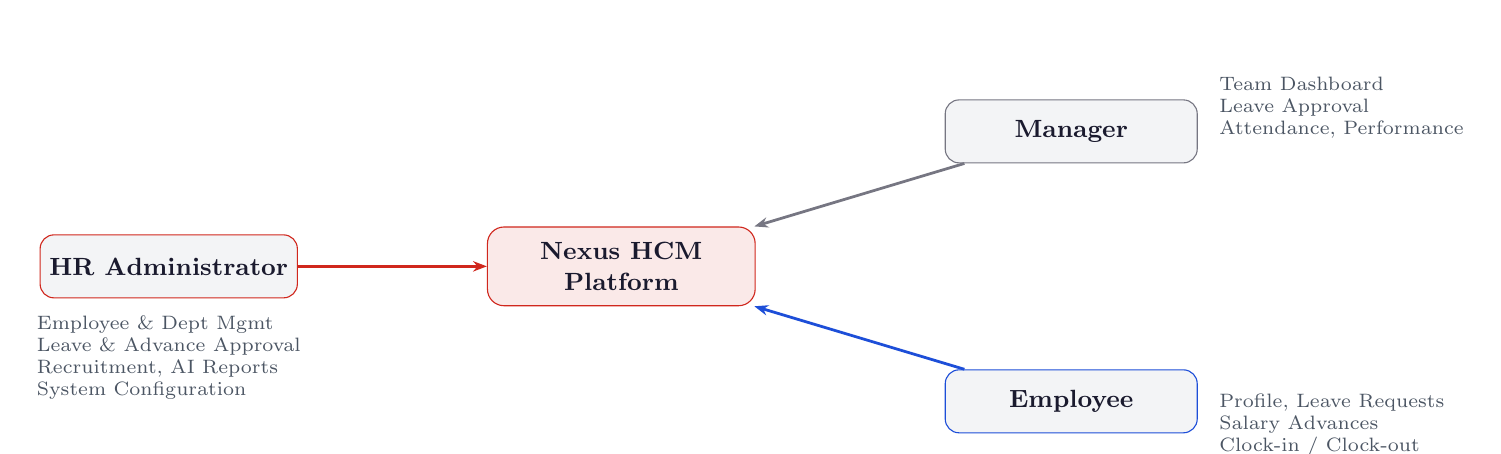
\begin{tikzpicture}[node distance=0.4cm and 1.8cm]

  %% Central platform node
  \node[draw=adpred, fill=adpred!10, rounded corners=6pt,
        minimum width=3.4cm, minimum height=1cm,
        align=center, font=\small\bfseries\color{adpdark}]
    (plat) {Nexus HCM\\Platform};

  %% HR Admin node
  \node[draw=adpred, fill=adplightgray, rounded corners=5pt,
        minimum width=3.2cm, minimum height=0.8cm,
        align=center, font=\small\bfseries\color{adpdark},
        left=2.4cm of plat] (admin) {HR Administrator};

  %% Manager node
  \node[draw=adpdark!60, fill=adplightgray, rounded corners=5pt,
        minimum width=3.2cm, minimum height=0.8cm,
        align=center, font=\small\bfseries\color{adpdark},
        above right=0.8cm and 2.4cm of plat] (mgr) {Manager};

  %% Employee node
  \node[draw=adpblue, fill=adplightgray, rounded corners=5pt,
        minimum width=3.2cm, minimum height=0.8cm,
        align=center, font=\small\bfseries\color{adpdark},
        below right=0.8cm and 2.4cm of plat] (emp) {Employee};

  %% Arrows
  \draw[-{Stealth[length=5pt]},color=adpred,line width=1pt] (admin) -- (plat);
  \draw[-{Stealth[length=5pt]},color=adpdark!60,line width=1pt] (mgr)  -- (plat);
  \draw[-{Stealth[length=5pt]},color=adpblue,line width=1pt]  (emp)   -- (plat);

  %% Feature annotations below each role
  \node[font=\scriptsize, text=adpgray, align=left, below=0.1cm of admin]
    {\scriptsize Employee \& Dept Mgmt\\
     \scriptsize Leave \& Advance Approval\\
     \scriptsize Recruitment, AI Reports\\
     \scriptsize System Configuration};

  \node[font=\scriptsize, text=adpgray, align=left, right=0.15cm of mgr,
        yshift=0.3cm]
    {\scriptsize Team Dashboard\\
     \scriptsize Leave Approval\\
     \scriptsize Attendance, Performance};

  \node[font=\scriptsize, text=adpgray, align=left, right=0.15cm of emp,
        yshift=-0.3cm]
    {\scriptsize Profile, Leave Requests\\
     \scriptsize Salary Advances\\
     \scriptsize Clock-in / Clock-out};

\end{tikzpicture}
\caption{Nexus HCM, User Roles and Responsibilities}
\label{fig:roles}
\end{figure}

\section{Study of Existing Solutions}

\subsection{Overview of Current HR Management Tools}

Before proposing a solution, a comparative analysis of existing HR management approaches
was conducted. The tools examined fall into three categories: manual approaches
(spreadsheets, email), standalone HR tools (single-module software), and integrated
HCM suites (SAP SuccessFactors, Oracle HCM, Workday).

\begin{itemize}
  \item \textbf{Spreadsheet-based management:} the most common approach in small and
    mid-sized companies. Offers no workflow automation, no access control, and no
    real-time visibility. Data integrity is entirely dependent on manual discipline.

  \item \textbf{Standalone HR Tools} (e.g., leave management apps, attendance trackers):
    address individual pain points but create new fragmentation. Data does not flow
    between modules, and reports must be assembled manually.

  \item \textbf{Enterprise HCM Suites} (SAP SuccessFactors, Oracle HCM, Workday):
    comprehensive and feature-rich, but prohibitively expensive for most Tunisian
    organizations, require heavy configuration, and are not adapted to local labor law
    or language requirements.
\end{itemize}

\subsection{Comparative Analysis}

\begin{table}[H]
\centering
\caption{Comparison of HR Management Approaches}
\label{tab:comparison}
\begin{tabular}{|L{3.8cm}|C{2.3cm}|C{2.5cm}|C{3.2cm}|}
\hline
\rowcolor{adpdark}
\textbf{\color{white}Feature} &
\textbf{\color{white}Spreadsheets} &
\textbf{\color{white}Standalone Tools} &
\textbf{\color{white}Nexus HCM} \\
\hline
Centralized employee data   & \xmark & Partial & \cmark \\
\hline
\rowcolor{adplightgray}
Leave approval workflow     & \xmark & Partial & \cmark \\
\hline
Digital attendance tracking & \xmark & Partial & \cmark \\
\hline
\rowcolor{adplightgray}
Role-based access control   & \xmark & Basic   & \cmark \\
\hline
Onboarding automation       & \xmark & \xmark  & \cmark \\
\hline
\rowcolor{adplightgray}
AI-powered reports          & \xmark & \xmark  & \cmark \\
\hline
Audit trail                 & \xmark & Partial & \cmark \\
\hline
\rowcolor{adplightgray}
Recruitment pipeline        & \xmark & \xmark  & \cmark \\
\hline
Cost                        & Free   & Moderate & Low (custom) \\
\hline
\end{tabular}
\end{table}

\subsection{Critique and Motivation}

The analysis reveals a clear gap in the market for a custom, affordable, and locally
adapted HR platform. Enterprise suites are too costly and generic. Standalone tools
create new silos. Spreadsheets offer no automation or security. \textbf{Nexus HCM} fills
this gap by providing a unified, role-driven platform specifically designed for the
operational context of the internship.

\section{Proposed Solution}

\textbf{Nexus HCM} is a centralized, web-based HR management platform that directly
addresses all identified weaknesses. It is built on a modern, decoupled architecture
with a \textbf{Spring Boot 3} REST backend and an \textbf{Angular 17} standalone-component
frontend, and includes the following core capabilities:

\begin{enumerate}
  \item \textbf{Employee Onboarding and Account Provisioning:} HR Admins create accounts
    via a dedicated form. The system automatically generates a secure activation token and
    sends an email containing a personalized setup link.
  \item \textbf{Role-Based Authentication and Navigation:} a JWT-secured login flow
    redirects each user to their role-specific dashboard upon authentication.
  \item \textbf{Department and Organizational Management:} departments are managed
    centrally, and an interactive org chart visualizes the full reporting hierarchy with
    collapsible subtrees.
  \item \textbf{Leave and Salary Advance Workflows:} structured approval pipelines with
    status tracking and in-app notification badges.
  \item \textbf{Attendance Tracking:} digital clock-in/clock-out with per-employee weekly
    calendar views for managers.
  \item \textbf{Performance Evaluation:} configurable evaluation campaigns with per-period
    scoring and manager-driven assessment.
  \item \textbf{Job Board and Recruitment Pipeline:} HR Admins manage job postings through
    a full lifecycle (DRAFT, OPEN, CLOSED). A public Careers page allows external candidates
    to apply with a CV attachment. Applications flow through a review pipeline.
  \item \textbf{AI-Powered HR Report Generation:} workforce metrics are aggregated and
    submitted to the OpenAI GPT-4 API, which returns a structured, natural-language
    executive HR report.
  \item \textbf{Dynamic System Configuration:} company branding (logo, name, primary
    color) is configurable at runtime and propagates to all pages instantly.
  \item \textbf{Audit Trail:} every HR action is logged with actor, timestamp, and
    description for full operational traceability.
\end{enumerate}

\section{Development Methodology}

\subsection{Methodology Selection}

Choosing the right project management methodology is critical to the success of a software
development project. Two main families of approaches exist: classical (Waterfall) methods
and Agile methods. Table~\ref{tab:methodology_comparison} summarizes their key differences.

\begin{table}[H]
\centering
\caption{Classical vs. Agile Methodology Comparison}
\label{tab:methodology_comparison}
\begin{tabular}{|L{4cm}|C{4cm}|C{4cm}|}
\hline
\rowcolor{adplightgray}
\textbf{Criterion}    & \textbf{Classical (Waterfall)} & \textbf{Agile (Scrum)} \\
\hline
Requirements          & Fixed upfront   & Evolving, iterative \\
\hline
Delivery              & Single final    & Incremental sprints \\
\hline
Client involvement    & At milestones   & Continuous \\
\hline
Adaptability to change & Low            & High \\
\hline
Risk management       & End-of-project  & Per sprint \\
\hline
Suited for            & Well-defined scope & Evolving requirements \\
\hline
\end{tabular}
\end{table}

\subsection{Adopted Methodology, Agile Scrum}

Given the iterative nature of this project and the need for continuous feedback from the
company supervisor, the \textbf{Agile Scrum} framework was adopted. Scrum organizes
development into fixed-length iterations called \textbf{Sprints}, each producing a
working, tested increment of the product.

\begin{figure}[H]
\centering
\includegraphics[width=0.82\textwidth]{scrum.png}
\caption{Agile Scrum Development Framework}
\label{fig:scrum}
\end{figure}

The key Scrum ceremonies applied during this internship were:
\begin{itemize}
  \item \textbf{Sprint Planning:} at the start of each sprint, tasks were selected from
    the product backlog and assigned to the sprint backlog.
  \item \textbf{Sprint Review:} at the end of each sprint, the completed features were
    demonstrated to the company supervisor for validation.
  \item \textbf{Sprint Retrospective:} lessons learned were discussed to improve the
    process for the next iteration.
\end{itemize}

\subsection{Sprint Planning Overview}

The internship (01 April, 30 September 2026) was organized into five sprints:

\begin{table}[H]
\centering
\caption{Sprint Planning, Nexus HCM}
\label{tab:sprints}
\begin{tabular}{|C{1.4cm}|C{3cm}|L{8.5cm}|}
\hline
\rowcolor{adpdark}
\textbf{\color{white}Sprint} &
\textbf{\color{white}Period} &
\textbf{\color{white}Delivered Features} \\
\hline
0 & 01/04, 14/04 &
  Environment setup, architecture design, database modeling, requirements analysis \\
\hline
\rowcolor{adplightgray}
1 & 15/04, 30/04 &
  Authentication (JWT), role-based routing, employee CRUD, department management,
  activation email, HR Admin dashboard \\
\hline
2 & 01/05, 31/05 &
  Organizational chart (collapsible tree), leave request workflow,
  attendance clock-in/out, salary advance management, performance evaluation \\
\hline
\rowcolor{adplightgray}
3 & 01/06, 31/07 &
  Job Board (HR panel), public Careers page, CV upload, application pipeline,
  AI-powered HR report generation, intelligent CV screening \\
\hline
4 & 01/08, 30/09 &
  Dynamic system configuration, audit trail, manager dashboard, employee
  self-service portal, testing, GitHub deployment \\
\hline
\end{tabular}
\end{table}

\section{Conclusion}

This chapter provided a comprehensive overview of the project framework. It introduced
ADP ES Tunisie, identified the limitations of current HR management practices, presented
Nexus HCM as a structured solution, analyzed comparable existing systems, and described
the Agile Scrum methodology driving the development process. The following chapters detail
the technical requirements, architecture, implementation, and validation of the platform.

\newpage

%%=======================================================================
%% CHAPTER 2
%%=======================================================================
\chapter{Requirements Specification}

\section{Introduction}

This chapter formalizes the requirements of the Nexus HCM platform. It identifies the
system actors, enumerates functional and non-functional requirements, and presents UML use
case diagrams modeling the interactions between each user profile and the system.

\section{System Actors}

A system actor is any entity that interacts with the application from outside its boundary.
Nexus HCM defines three primary actors and one external actor:

\begin{table}[H]
\centering
\caption{System Actors Description}
\label{tab:actors}
\begin{tabular}{|C{3.2cm}|L{10cm}|}
\hline
\rowcolor{adplightgray}
\textbf{Actor} & \textbf{Description and Responsibilities} \\
\hline
\textbf{HR Administrator} &
  The most privileged internal user. Manages the complete employee lifecycle, all
  departments, leave approvals, salary advance reviews, job postings, performance
  campaigns, AI report generation, and platform configuration. \\
\hline
\textbf{Manager} &
  Supervises a team of direct reports. Reviews and approves team leave requests,
  monitors attendance, conducts performance evaluations, and consults team
  dashboards. \\
\hline
\textbf{Employee} &
  Standard internal user. Views and updates personal profile, submits leave and
  salary advance requests, performs clock-in/clock-out, and consults personal
  performance results. \\
\hline
\textbf{Candidate (Public)} &
  External actor, no login required. Browses open job positions on the public
  Careers page and submits applications with CV attachment. \\
\hline
\end{tabular}
\end{table}

\section{Functional Requirements}

\subsection{Authentication and Access Control}
\begin{itemize}
  \item The system shall authenticate users via email/password credentials.
  \item On successful login, users shall be redirected to their role-specific dashboard
    (HR Admin to \texttt{/dashboard}, Manager to \texttt{/manager-dashboard}, Employee
    to \texttt{/my-dashboard}).
  \item All API endpoints shall be protected by a stateless JWT authentication mechanism.
  \item The system shall support secure account activation through a tokenized email link.
  \item Session tokens shall expire after a configurable timeout period.
\end{itemize}

\subsection{Employee Management}
\begin{itemize}
  \item HR Admins shall create, read, update, and deactivate employee accounts.
  \item Each employee shall be assigned a role (HR\_ADMIN, MANAGER, EMPLOYEE),
    a department, and optionally a reporting manager.
  \item The system shall send an automated activation email on account creation.
  \item HR Admins shall reassign reporting managers to any employee at any time.
\end{itemize}

\subsection{Department Management}
\begin{itemize}
  \item HR Admins shall create, rename, and delete departments.
  \item Each employee shall belong to exactly one department.
  \item The system shall display employee distribution per department.
\end{itemize}

\subsection{Organizational Chart}
\begin{itemize}
  \item The system shall render a hierarchical org chart based on manager-employee
    reporting relationships.
  \item Each node shall be collapsible/expandable to show or hide its subtree.
  \item The chart shall support name-based search with visual highlighting.
  \item HR Admins shall reassign manager relationships directly from the chart view.
\end{itemize}

\subsection{Leave Request Management}
\begin{itemize}
  \item Employees shall submit leave requests specifying type, date range, and reason.
  \item Managers and HR Admins shall approve or reject pending requests with
    optional reviewer notes.
  \item Requests shall follow the status workflow: PENDING, APPROVED, REJECTED.
  \item The HR Admin dashboard shall display a badge with the count of pending requests.
\end{itemize}

\subsection{Attendance Tracking}
\begin{itemize}
  \item Employees shall record their daily presence via a clock-in/clock-out mechanism.
  \item The system shall store the exact timestamp of each event.
  \item Managers shall view their team's weekly attendance calendar.
\end{itemize}

\subsection{Salary Advance Management}
\begin{itemize}
  \item Employees shall submit salary advance requests with amount and justification.
  \item HR Admins shall approve or reject requests with optional notes.
  \item The dashboard shall display a pending advance count badge.
\end{itemize}

\subsection{Performance Evaluation}
\begin{itemize}
  \item HR Admins shall create evaluation campaigns with configurable questionnaires.
  \item Managers shall submit evaluations for their direct reports per period.
  \item Evaluation results shall be persisted per employee, per period.
\end{itemize}

\subsection{Job Board and Recruitment}
\begin{itemize}
  \item HR Admins shall create job positions and manage their lifecycle
    (DRAFT, OPEN, CLOSED).
  \item OPEN positions shall appear on the public Careers page without login.
  \item External candidates shall apply online with name, email, cover letter,
    and optional CV file (PDF, DOC, DOCX, max 5 MB).
  \item HR Admins shall move applications through a pipeline
    (NEW, REVIEWING, INTERVIEW, REJECTED, ACCEPTED).
\end{itemize}

\subsection{AI-Powered HR Report Generation}
\begin{itemize}
  \item HR Admins shall trigger report generation with a single click.
  \item The system shall aggregate workforce metrics (employee counts, leave rates,
    attendance patterns, department breakdown) into a structured prompt.
  \item The prompt shall be submitted to the OpenAI GPT-4 API.
  \item The returned natural-language report shall be displayed in the dashboard.
\end{itemize}

\subsection{System Configuration}
\begin{itemize}
  \item HR Admins shall update platform branding (company name, logo URL, primary color).
  \item Configuration changes shall propagate in real time to all pages, including
    the public login and careers pages.
  \item Configuration values shall persist in the database across server restarts.
\end{itemize}

\section{Non-Functional Requirements}

\begin{table}[H]
\centering
\caption{Non-Functional Requirements}
\label{tab:nfr}
\begin{tabular}{|C{3cm}|L{10cm}|}
\hline
\rowcolor{adplightgray}
\textbf{Category} & \textbf{Requirement} \\
\hline
\textbf{Security} &
  All endpoints protected by JWT. Passwords stored using BCrypt hashing.
  RBAC enforced at both backend controller and frontend routing levels. \\
\hline
\textbf{Performance} &
  Standard CRUD responses under 300 ms. Statistics computed server-side
  to minimize client-side processing overhead. \\
\hline
\textbf{Usability} &
  Responsive, modern UI. Role-specific dashboards reduce cognitive load.
  Toast notifications for all user actions. \\
\hline
\textbf{Maintainability} &
  Layered Spring Boot architecture (Controller, Service, Repository).
  Standalone Angular components with no NgModule dependencies.
  Descriptive Git commits, full source on GitHub. \\
\hline
\textbf{Scalability} &
  Stateless REST API supports horizontal scaling.
  Normalized MySQL schema designed to accommodate organizational growth. \\
\hline
\textbf{Availability} &
  Deployable on any Java-capable server.
  Hibernate DDL auto-update creates and migrates schema on startup. \\
\hline
\end{tabular}
\end{table}

\section{Use Case Diagrams}

\subsection{Global Use Case Diagram}

\begin{figure}[H]
\centering
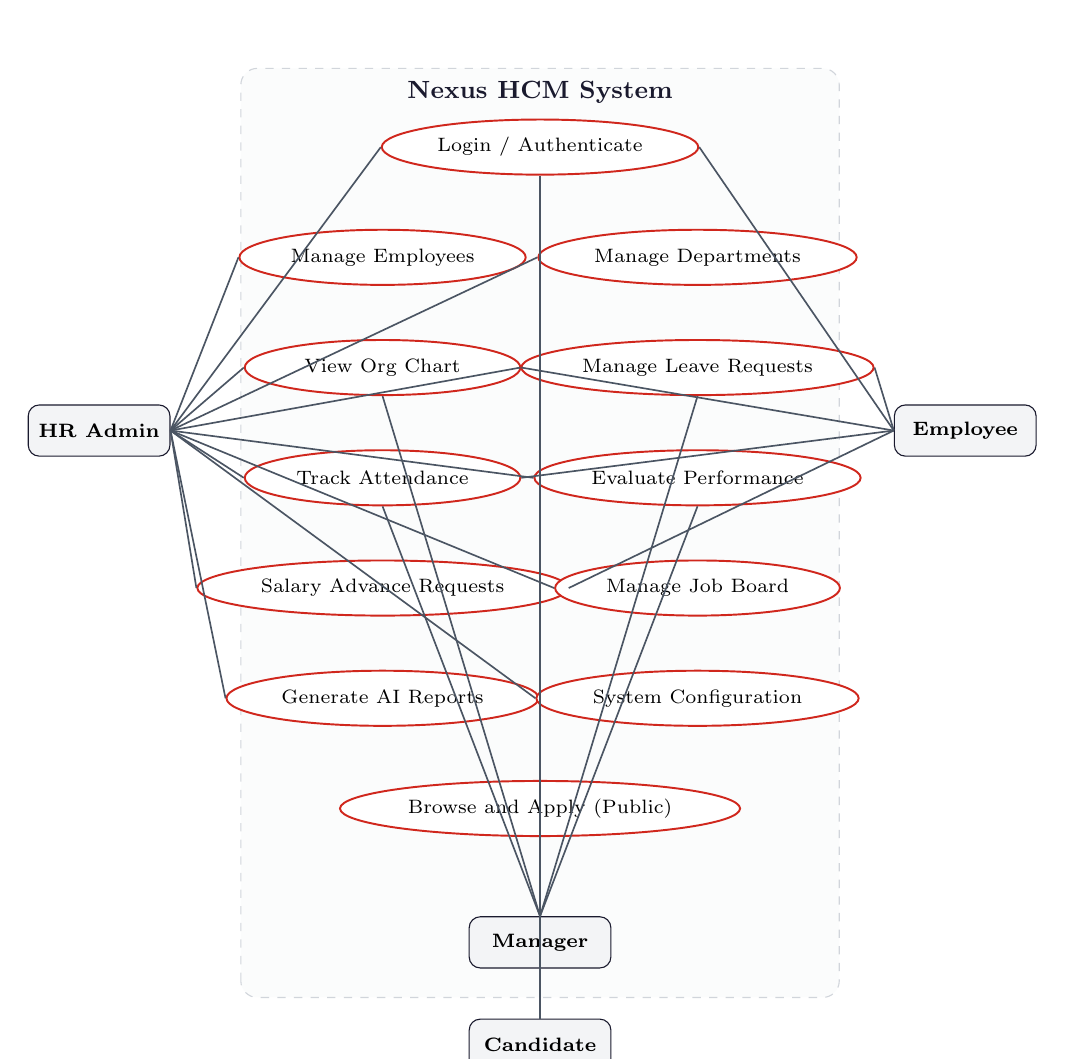
\begin{tikzpicture}[
  every node/.style={font=\small},
  uc/.style={draw=adpred, ellipse, fill=white, minimum width=3.5cm,
             minimum height=0.7cm, align=center, line width=0.7pt,
             font=\scriptsize},
  act/.style={draw=adpdark, fill=adplightgray, rounded corners=4pt,
              minimum width=1.8cm, minimum height=0.65cm,
              align=center, font=\scriptsize\bfseries},
  assoc/.style={draw=adpgray, line width=0.6pt}
]

%% System boundary
\draw[draw=adpborder, dashed, fill=adplightgray!30, rounded corners=6pt]
  (0.6,-0.2) rectangle (8.2,11.6);
\node[font=\small\bfseries, text=adpdark] at (4.4,11.3) {Nexus HCM System};

%% Use cases (inside boundary)
\node[uc] (login)  at (4.4,10.6) {Login / Authenticate};
\node[uc] (empm)   at (2.4,9.2)  {Manage Employees};
\node[uc] (deptm)  at (6.4,9.2)  {Manage Departments};
\node[uc] (org)    at (2.4,7.8)  {View Org Chart};
\node[uc] (leave)  at (6.4,7.8)  {Manage Leave Requests};
\node[uc] (attend) at (2.4,6.4)  {Track Attendance};
\node[uc] (perf)   at (6.4,6.4)  {Evaluate Performance};
\node[uc] (adv)    at (2.4,5.0)  {Salary Advance Requests};
\node[uc] (job)    at (6.4,5.0)  {Manage Job Board};
\node[uc] (report) at (2.4,3.6)  {Generate AI Reports};
\node[uc] (config) at (6.4,3.6)  {System Configuration};
\node[uc] (career) at (4.4,2.2)  {Browse and Apply (Public)};

%% Actors
\node[act] (hradmin) at (-1.2,7.0) {HR Admin};
\node[act] (mgr)     at (4.4,0.5)  {Manager};
\node[act] (empa)    at (9.8,7.0)  {Employee};
\node[act] (pub)     at (4.4,-0.8) {Candidate};

%% HR Admin associations
\foreach \uc in {login,empm,deptm,org,leave,attend,perf,adv,job,report,config}
  \draw[assoc] (hradmin.east) -- (\uc.west);

%% Manager associations
\foreach \uc in {login,org,leave,attend,perf}
  \draw[assoc] (mgr.north) -- (\uc.south);

%% Employee associations
\foreach \uc in {login,org,leave,attend,adv}
  \draw[assoc] (empa.west) -- (\uc.east);

%% Public candidate
\draw[assoc] (pub.north) -- (career.south);

\end{tikzpicture}
\caption{Global Use Case Diagram, Nexus HCM}
\label{fig:global_uc}
\end{figure}

\subsection{HR Admin Use Case Detail}

\begin{figure}[H]
\centering
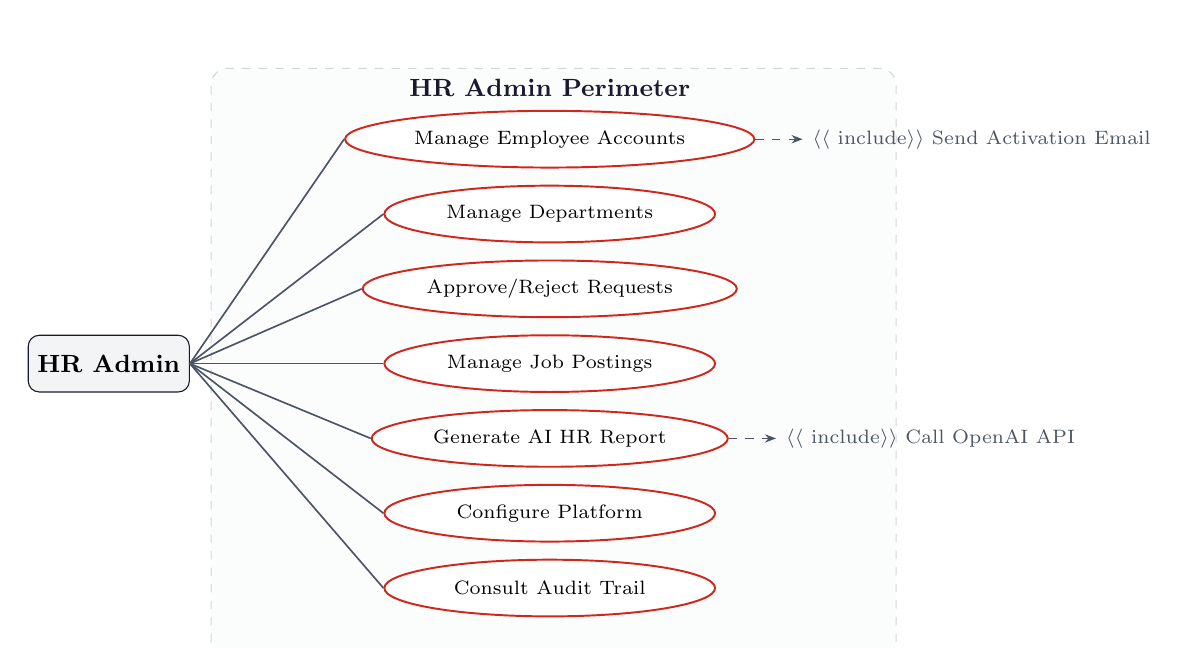
\begin{tikzpicture}[
  uc/.style={draw=adpred, ellipse, fill=white, minimum width=4.2cm,
             minimum height=0.72cm, align=center,
             line width=0.7pt, font=\scriptsize},
  act/.style={draw=adpdark, fill=adplightgray, rounded corners=4pt,
              minimum width=2cm, minimum height=0.72cm,
              align=center, font=\small\bfseries},
  assoc/.style={draw=adpgray, line width=0.6pt}
]
\draw[draw=adpborder,dashed,fill=adplightgray!30,rounded corners=6pt]
  (0.3,-0.3) rectangle (9.0,7.2);
\node[font=\small\bfseries, text=adpdark] at (4.6,6.95) {HR Admin Perimeter};

\node[uc] (e1) at (4.6,6.3) {Manage Employee Accounts};
\node[uc] (e2) at (4.6,5.35){Manage Departments};
\node[uc] (e3) at (4.6,4.4) {Approve/Reject Requests};
\node[uc] (e4) at (4.6,3.45){Manage Job Postings};
\node[uc] (e5) at (4.6,2.5) {Generate AI HR Report};
\node[uc] (e6) at (4.6,1.55){Configure Platform};
\node[uc] (e7) at (4.6,0.6) {Consult Audit Trail};

\node[act] (admin) at (-1.0,3.45) {HR Admin};
\foreach \n in {e1,e2,e3,e4,e5,e6,e7}
  \draw[assoc] (admin.east) -- (\n.west);

%% Include relationships
\draw[draw=adpgray,dashed,-{Stealth[length=4pt]}] (e1.east)
  -- ++(0.6,0) node[right,font=\scriptsize\color{adpgray}]
  {$\langle\langle$ include$\rangle\rangle$\ Send Activation Email};
\draw[draw=adpgray,dashed,-{Stealth[length=4pt]}] (e5.east)
  -- ++(0.6,0) node[right,font=\scriptsize\color{adpgray}]
  {$\langle\langle$ include$\rangle\rangle$\ Call OpenAI API};

\end{tikzpicture}
\caption{HR Administrator Use Case Diagram}
\label{fig:uc_admin}
\end{figure}

\subsection{Employee Use Case Detail}

\begin{figure}[H]
\centering
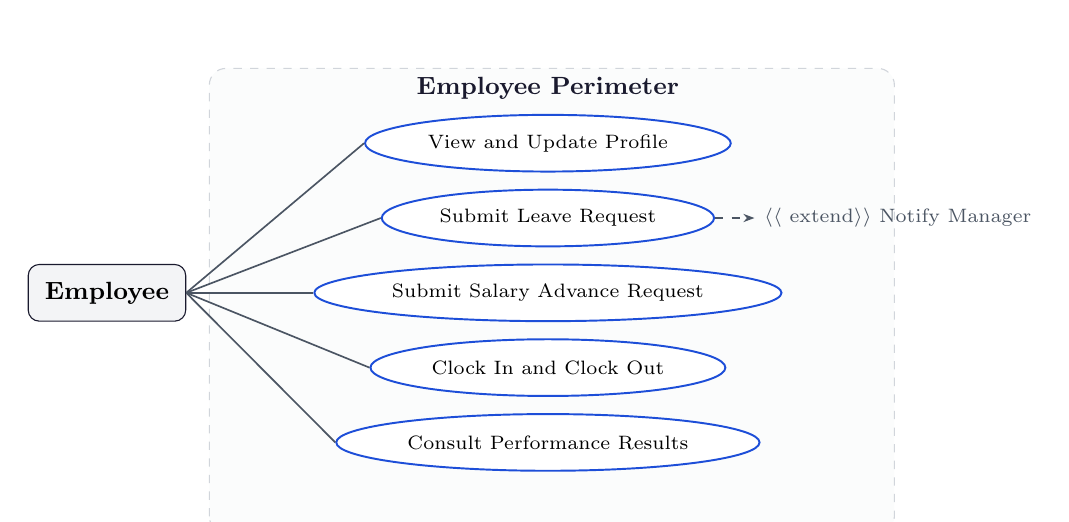
\begin{tikzpicture}[
  uc/.style={draw=adpblue, ellipse, fill=white, minimum width=4.2cm,
             minimum height=0.72cm, align=center,
             line width=0.7pt, font=\scriptsize},
  act/.style={draw=adpdark, fill=adplightgray, rounded corners=4pt,
              minimum width=2cm, minimum height=0.72cm,
              align=center, font=\small\bfseries},
  assoc/.style={draw=adpgray, line width=0.6pt}
]
\draw[draw=adpborder,dashed,fill=adplightgray!30,rounded corners=6pt]
  (0.3,-0.3) rectangle (9.0,5.6);
\node[font=\small\bfseries, text=adpdark] at (4.6,5.35) {Employee Perimeter};

\node[uc] (u1) at (4.6,4.65) {View and Update Profile};
\node[uc] (u2) at (4.6,3.7)  {Submit Leave Request};
\node[uc] (u3) at (4.6,2.75) {Submit Salary Advance Request};
\node[uc] (u4) at (4.6,1.8)  {Clock In and Clock Out};
\node[uc] (u5) at (4.6,0.85) {Consult Performance Results};

\node[act] (empa) at (-1.0,2.75) {Employee};
\foreach \n in {u1,u2,u3,u4,u5}
  \draw[assoc] (empa.east) -- (\n.west);

%% Extend
\draw[draw=adpgray,dashed,-{Stealth[length=4pt]}] (u2.east)
  -- ++(0.5,0) node[right,font=\scriptsize, text=adpgray]
  {$\langle\langle$ extend$\rangle\rangle$\ Notify Manager};

\end{tikzpicture}
\caption{Employee Use Case Diagram}
\label{fig:uc_employee}
\end{figure}

\section{Conclusion}

This chapter provided a complete specification of Nexus HCM requirements. The four actors,
their roles, and their interactions with the system have been formalized through functional
and non-functional requirements and three UML use case diagrams. These specifications
constitute the contractual baseline for all architectural and implementation decisions
described in the following chapters.

\newpage


%%=======================================================================
%% CHAPTER 3 -- ARCHITECTURE AND DESIGN
%%=======================================================================
\chapter{System Architecture and Design}

\section{Introduction}

This chapter presents the technical architecture of Nexus HCM. It describes the
three-tier architectural pattern, the full technology stack, the UML class diagram
of the domain model, key sequence diagrams, the database entity-relationship schema,
and the deployment architecture.

\section{Software Architecture}

\subsection{Three-Tier Architecture}

Nexus HCM follows a classic \textbf{three-tier architecture} that physically separates
the presentation layer, business logic layer, and data layer. This separation promotes
modularity, testability, and the ability for each tier to evolve independently.

\begin{figure}[H]
\centering
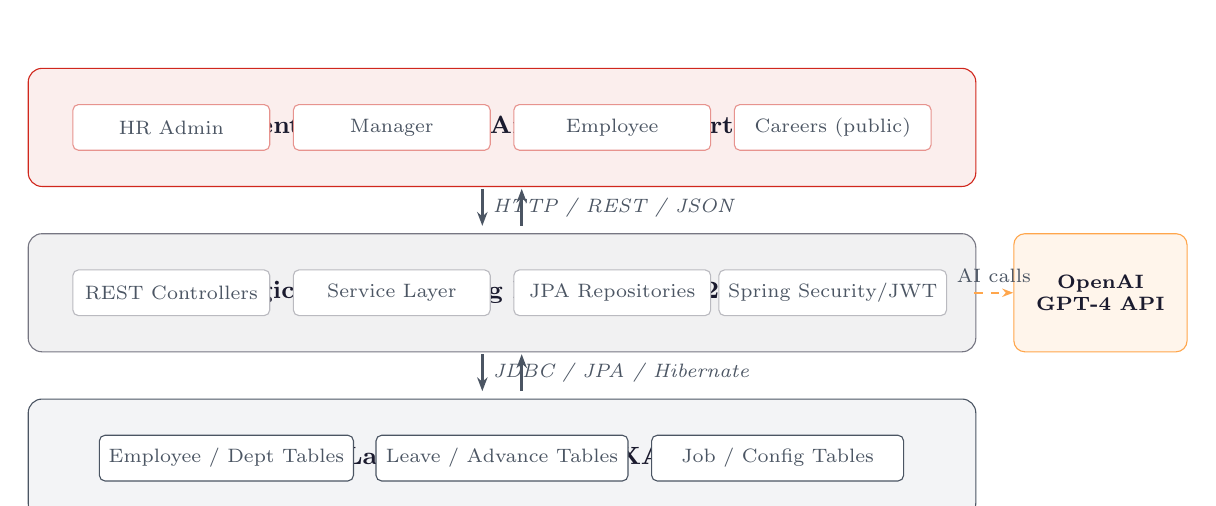
\begin{tikzpicture}[node distance=0.5cm]

  %% Tier 1: Presentation
  \node[draw=adpred, fill=adpred!8, rounded corners=5pt,
        minimum width=12cm, minimum height=1.5cm,
        text width=11.8cm, align=center,
        font=\small\bfseries\color{adpdark}]
    (pres) at (0,0) {Presentation Layer \quad Angular 17 \quad Port 4200};

  \node[draw=adpred!50, fill=white, rounded corners=2pt,
        minimum width=2.5cm, minimum height=0.58cm,
        align=center, font=\scriptsize\color{adpgray}]
    (p1) at (-4.2,-0.0) {};
  \node[font=\scriptsize\color{adpgray}] at (-4.2,0) {HR Admin};

  \node[draw=adpred!50, fill=white, rounded corners=2pt,
        minimum width=2.5cm, minimum height=0.58cm,
        align=center, font=\scriptsize\color{adpgray}]
    at (-1.4,0) {Manager};
  \node[draw=adpred!50, fill=white, rounded corners=2pt,
        minimum width=2.5cm, minimum height=0.58cm,
        align=center, font=\scriptsize\color{adpgray}]
    at (1.4,0)  {Employee};
  \node[draw=adpred!50, fill=white, rounded corners=2pt,
        minimum width=2.5cm, minimum height=0.58cm,
        align=center, font=\scriptsize\color{adpgray}]
    at (4.2,0)  {Careers (public)};

  %% Arrow 1
  \draw[-{Stealth[length=5pt]},draw=adpgray,line width=0.9pt]
    (-0.25,-0.78) -- (-0.25,-1.25)
    node[midway,right,font=\scriptsize\itshape\color{adpgray}]
    {HTTP / REST / JSON};
  \draw[-{Stealth[length=5pt]},draw=adpgray,line width=0.9pt]
    (0.25,-1.25) -- (0.25,-0.78);

  %% Tier 2: Business Logic
  \node[draw=adpdark!60, fill=adpdark!6, rounded corners=5pt,
        minimum width=12cm, minimum height=1.5cm,
        text width=11.8cm, align=center,
        font=\small\bfseries\color{adpdark}]
    (biz) at (0,-2.1) {Business Logic Layer \quad Spring Boot 3 / Java 21 \quad Port 8085};

  \node[draw=adpdark!30, fill=white, rounded corners=2pt,
        minimum width=2.5cm, minimum height=0.58cm,
        align=center, font=\scriptsize\color{adpgray}]
    at (-4.2,-2.1) {REST Controllers};
  \node[draw=adpdark!30, fill=white, rounded corners=2pt,
        minimum width=2.5cm, minimum height=0.58cm,
        align=center, font=\scriptsize\color{adpgray}]
    at (-1.4,-2.1) {Service Layer};
  \node[draw=adpdark!30, fill=white, rounded corners=2pt,
        minimum width=2.5cm, minimum height=0.58cm,
        align=center, font=\scriptsize\color{adpgray}]
    at (1.4,-2.1)  {JPA Repositories};
  \node[draw=adpdark!30, fill=white, rounded corners=2pt,
        minimum width=2.5cm, minimum height=0.58cm,
        align=center, font=\scriptsize\color{adpgray}]
    at (4.2,-2.1)  {Spring Security/JWT};

  %% External AI
  \node[draw=orange!70, fill=orange!8, rounded corners=4pt,
        minimum width=2.2cm, minimum height=1.5cm,
        align=center, font=\scriptsize\bfseries\color{adpdark}]
    (ai) at (7.6,-2.1) {OpenAI\\GPT-4 API};
  \draw[-{Stealth[length=4pt]},draw=orange!70,line width=0.8pt,dashed]
    (6.0,-2.1) -- (ai.west)
    node[midway,above,font=\scriptsize\color{adpgray}]{AI calls};

  %% Arrow 2
  \draw[-{Stealth[length=5pt]},draw=adpgray,line width=0.9pt]
    (-0.25,-2.88) -- (-0.25,-3.35)
    node[midway,right,font=\scriptsize\itshape\color{adpgray}]
    {JDBC / JPA / Hibernate};
  \draw[-{Stealth[length=5pt]},draw=adpgray,line width=0.9pt]
    (0.25,-3.35) -- (0.25,-2.88);

  %% Tier 3: Data
  \node[draw=adpgray, fill=adplightgray, rounded corners=5pt,
        minimum width=12cm, minimum height=1.5cm,
        text width=11.8cm, align=center,
        font=\small\bfseries\color{adpdark}]
    (data) at (0,-4.2) {Data Layer \quad MySQL 8 / XAMPP};

  \node[draw=adpgray, fill=white, rounded corners=2pt,
        minimum width=3.2cm, minimum height=0.58cm,
        align=center, font=\scriptsize\color{adpgray}]
    at (-3.5,-4.2) {Employee / Dept Tables};
  \node[draw=adpgray, fill=white, rounded corners=2pt,
        minimum width=3.2cm, minimum height=0.58cm,
        align=center, font=\scriptsize\color{adpgray}]
    at (0,-4.2)    {Leave / Advance Tables};
  \node[draw=adpgray, fill=white, rounded corners=2pt,
        minimum width=3.2cm, minimum height=0.58cm,
        align=center, font=\scriptsize\color{adpgray}]
    at (3.5,-4.2)  {Job / Config Tables};

\end{tikzpicture}
\caption{Nexus HCM, Three-Tier System Architecture}
\label{fig:architecture}
\end{figure}

\subsection{Backend Layered Architecture}

The Spring Boot backend strictly follows the Controller, Service, Repository pattern.

\begin{figure}[H]
\centering
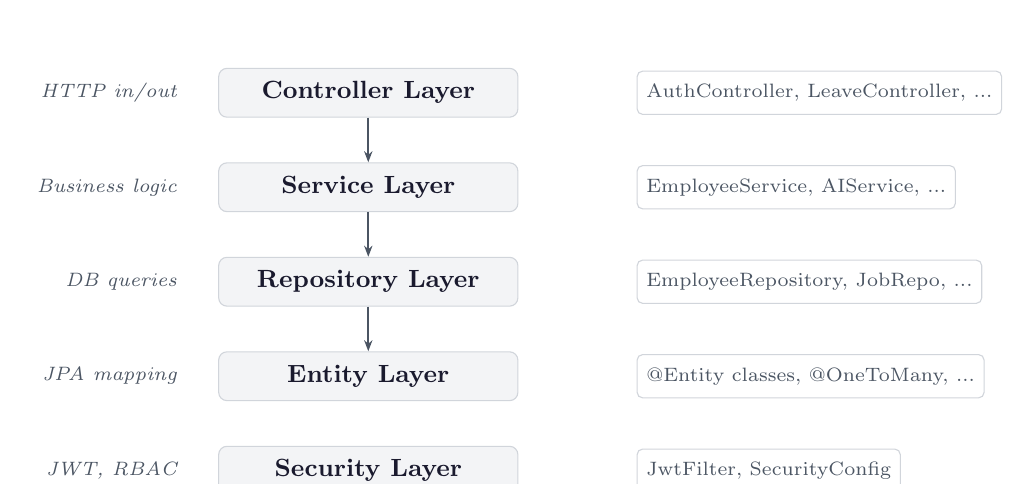
\begin{tikzpicture}[
  layer/.style={draw=adpborder, fill=adplightgray, rounded corners=3pt,
                minimum width=3.8cm, minimum height=0.62cm,
                align=center, font=\small\bfseries\color{adpdark}},
  detail/.style={draw=adpborder, fill=white, rounded corners=2pt,
                 minimum width=3.0cm, minimum height=0.55cm,
                 align=center, font=\scriptsize\color{adpgray}},
  arr/.style={-{Stealth[length=4pt]},draw=adpgray,line width=0.65pt}
]
  \node[layer] (c) at (0,5.4) {Controller Layer};
  \node[layer] (s) at (0,4.2) {Service Layer};
  \node[layer] (r) at (0,3.0) {Repository Layer};
  \node[layer] (e) at (0,1.8) {Entity Layer};
  \node[layer] (k) at (0,0.6) {Security Layer};

  \draw[arr] (c) -- (s);
  \draw[arr] (s) -- (r);
  \draw[arr] (r) -- (e);

  \node[detail, right=1.5cm of c] {AuthController, LeaveController, ...};
  \node[detail, right=1.5cm of s] {EmployeeService, AIService, ...};
  \node[detail, right=1.5cm of r] {EmployeeRepository, JobRepo, ...};
  \node[detail, right=1.5cm of e] {@Entity classes, @OneToMany, ...};
  \node[detail, right=1.5cm of k] {JwtFilter, SecurityConfig};

  \node[left=0.4cm of c, font=\scriptsize\itshape\color{adpgray}]
    {HTTP in/out};
  \node[left=0.4cm of s, font=\scriptsize\itshape\color{adpgray}]
    {Business logic};
  \node[left=0.4cm of r, font=\scriptsize\itshape\color{adpgray}]
    {DB queries};
  \node[left=0.4cm of e, font=\scriptsize\itshape\color{adpgray}]
    {JPA mapping};
  \node[left=0.4cm of k, font=\scriptsize\itshape\color{adpgray}]
    {JWT, RBAC};

\end{tikzpicture}
\caption{Spring Boot Backend, Layered Architecture}
\label{fig:backend_layers}
\end{figure}

\section{Technology Stack}

\begin{table}[H]
\centering
\caption{Technology Stack, Nexus HCM}
\label{tab:tech_stack}
\begin{tabular}{|C{2.2cm}|C{3.5cm}|L{7.5cm}|}
\hline
\rowcolor{adplightgray}
\textbf{Layer} & \textbf{Technology} & \textbf{Role} \\
\hline
\multirow{4}{*}{Backend}
  & Java 21             & Core programming language \\
  & Spring Boot 3.3     & Application framework, REST API, security \\
  & Spring Data JPA     & ORM and database abstraction (Hibernate) \\
  & Spring Security     & Authentication, authorization, JWT filter \\
\hline
\multirow{3}{*}{Frontend}
  & Angular 17          & SPA framework, standalone components \\
  & TypeScript          & Typed JavaScript superset \\
  & RxJS                & Reactive programming (Observables) \\
\hline
\multirow{2}{*}{Database}
  & MySQL 8             & Relational data storage \\
  & XAMPP               & Local development DB server \\
\hline
\multirow{4}{*}{Tools}
  & Lombok              & Java boilerplate reduction \\
  & Maven               & Build and dependency management \\
  & Postman             & API testing \\
  & GitHub              & Version control and deployment \\
\hline
\multirow{2}{*}{AI}
  & OpenAI GPT-4 API    & HR report generation, CV screening \\
  & Spring RestTemplate & HTTP client for AI API calls \\
\hline
\end{tabular}
\end{table}

\section{UML Class Diagram}

\begin{figure}[H]
\centering
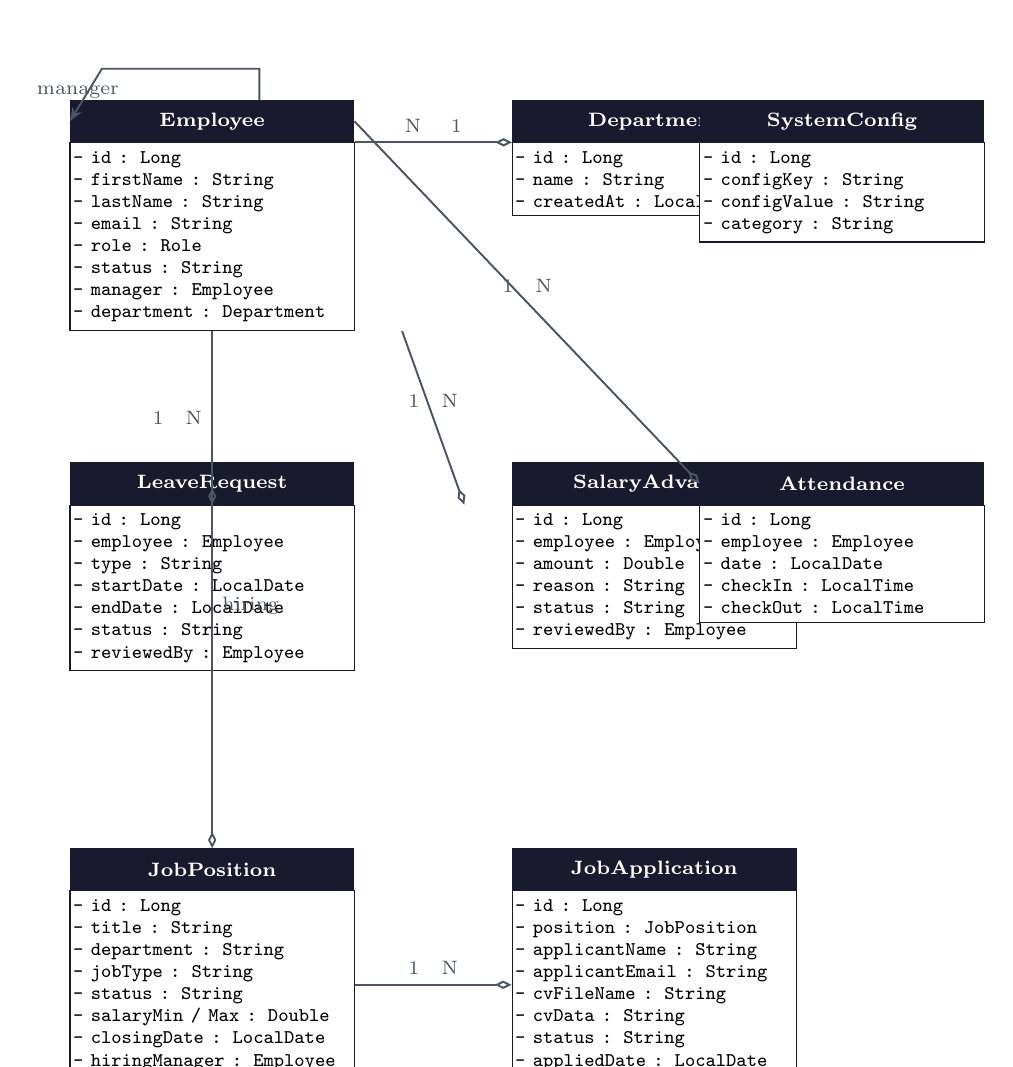
\begin{tikzpicture}[node distance=0pt]

  %% ---- Employee ----
  \node[umlheader] (e_h) at (0,0) {Employee};
  \node[umlattrbox, below=0pt of e_h] (e_a) {
    \texttt{- id : Long}\\
    \texttt{- firstName : String}\\
    \texttt{- lastName : String}\\
    \texttt{- email : String}\\
    \texttt{- role : Role}\\
    \texttt{- status : String}\\
    \texttt{- manager : Employee}\\
    \texttt{- department : Department}
  };

  %% ---- Department ----
  \node[umlheader, right=2.0cm of e_h] (d_h) {Department};
  \node[umlattrbox, below=0pt of d_h] (d_a) {
    \texttt{- id : Long}\\
    \texttt{- name : String}\\
    \texttt{- createdAt : LocalDate}
  };

  %% ---- LeaveRequest ----
  \node[umlheader] (l_h) at (0,-4.6) {LeaveRequest};
  \node[umlattrbox, below=0pt of l_h] (l_a) {
    \texttt{- id : Long}\\
    \texttt{- employee : Employee}\\
    \texttt{- type : String}\\
    \texttt{- startDate : LocalDate}\\
    \texttt{- endDate : LocalDate}\\
    \texttt{- status : String}\\
    \texttt{- reviewedBy : Employee}
  };

  %% ---- SalaryAdvance ----
  \node[umlheader, right=2.0cm of l_h] (s_h) {SalaryAdvance};
  \node[umlattrbox, below=0pt of s_h] (s_a) {
    \texttt{- id : Long}\\
    \texttt{- employee : Employee}\\
    \texttt{- amount : Double}\\
    \texttt{- reason : String}\\
    \texttt{- status : String}\\
    \texttt{- reviewedBy : Employee}
  };

  %% ---- JobPosition ----
  \node[umlheader] (j_h) at (0,-9.5) {JobPosition};
  \node[umlattrbox, below=0pt of j_h] (j_a) {
    \texttt{- id : Long}\\
    \texttt{- title : String}\\
    \texttt{- department : String}\\
    \texttt{- jobType : String}\\
    \texttt{- status : String}\\
    \texttt{- salaryMin / Max : Double}\\
    \texttt{- closingDate : LocalDate}\\
    \texttt{- hiringManager : Employee}
  };

  %% ---- JobApplication ----
  \node[umlheader, right=2.0cm of j_h] (a_h) {JobApplication};
  \node[umlattrbox, below=0pt of a_h] (a_a) {
    \texttt{- id : Long}\\
    \texttt{- position : JobPosition}\\
    \texttt{- applicantName : String}\\
    \texttt{- applicantEmail : String}\\
    \texttt{- cvFileName : String}\\
    \texttt{- cvData : String}\\
    \texttt{- status : String}\\
    \texttt{- appliedDate : LocalDate}
  };

  %% ---- SystemConfig ----
  \node[umlheader] (c_h) at (8.0,0) {SystemConfig};
  \node[umlattrbox, below=0pt of c_h] (c_a) {
    \texttt{- id : Long}\\
    \texttt{- configKey : String}\\
    \texttt{- configValue : String}\\
    \texttt{- category : String}
  };

  %% ---- Attendance ----
  \node[umlheader] (at_h) at (8.0,-4.6) {Attendance};
  \node[umlattrbox, below=0pt of at_h] (at_a) {
    \texttt{- id : Long}\\
    \texttt{- employee : Employee}\\
    \texttt{- date : LocalDate}\\
    \texttt{- checkIn : LocalTime}\\
    \texttt{- checkOut : LocalTime}
  };

  %% Relationships
  \draw[umlass] (e_a.north east) -- (d_h.south west)
    node[midway,above,font=\scriptsize\color{adpgray}]{N \quad 1};

  \draw[umlrel] ([xshift=0.6cm]e_h.north) -- ++(0,0.4)
    -- ++(-2.0,0) -- (e_h.west)
    node[near end,above,font=\scriptsize\color{adpgray}]{manager};

  \draw[umlass] (e_a.south) -- (l_a.north)
    node[midway,left,font=\scriptsize\color{adpgray}]{1\quad N};

  \draw[umlass] ([xshift=0.6cm]e_a.south east)
    -- ([xshift=-0.6cm]s_a.north west)
    node[midway,above,font=\scriptsize\color{adpgray}]{1\quad N};

  \draw[umlass] (e_h.east) -- (at_h.west)
    node[midway,above,font=\scriptsize\color{adpgray}]{1\quad N};

  \draw[umlass] (e_a.south) -- ++(0,-0.4) -| (j_h.north)
    node[near end,right,font=\scriptsize\color{adpgray}]{hiring};

  \draw[umlass] (j_a.east) -- (a_a.west)
    node[midway,above,font=\scriptsize\color{adpgray}]{1\quad N};

\end{tikzpicture}
\caption{UML Class Diagram, Nexus HCM Domain Model}
\label{fig:class_diagram}
\end{figure}

\section{Sequence Diagrams}

\subsection{Authentication Sequence}

\begin{figure}[H]
\centering
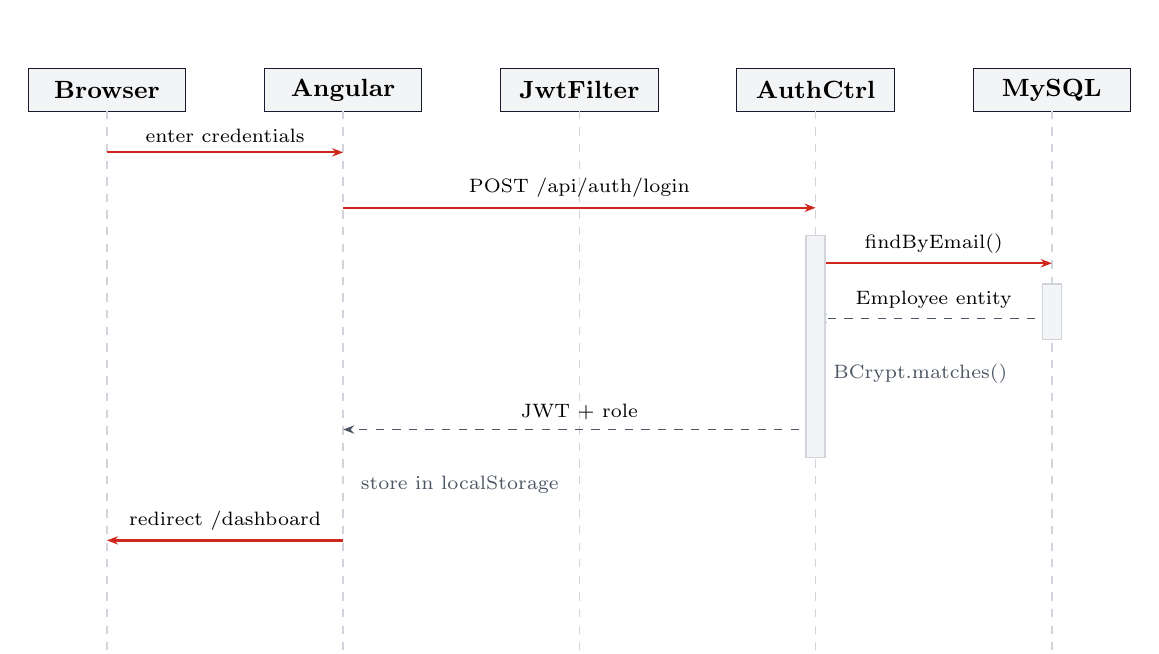
\begin{tikzpicture}[xscale=1.0, yscale=0.88]
  \node[seqobj] (browser) at (0.0,8) {Browser};
  \node[seqobj] (angular) at (3.0,8) {Angular};
  \node[seqobj] (filter)  at (6.0,8) {JwtFilter};
  \node[seqobj] (auth)    at (9.0,8) {AuthCtrl};
  \node[seqobj] (db)      at (12.0,8){MySQL};

  \foreach \x in {0,3,6,9,12}
    \draw[draw=adpborder,dashed,line width=0.5pt] (\x,7.7) -- (\x,-0.3);

  \draw[seqmsg] (0,7.1) -- (3,7.1)
    node[midway,above,font=\scriptsize]{enter credentials};
  \draw[seqmsg] (3,6.3) -- (9,6.3)
    node[midway,above,font=\scriptsize]{POST /api/auth/login};
  \draw[seqmsg] (9,5.5) -- (12,5.5)
    node[midway,above,font=\scriptsize]{findByEmail()};
  \draw[seqret] (12,4.7) -- (9,4.7)
    node[midway,above,font=\scriptsize]{Employee entity};
  \draw[seqmsg] (9,3.9) -- (9,3.9) ;
  \node[right,font=\scriptsize\color{adpgray}] at (9.1,3.9) {BCrypt.matches()};
  \draw[seqret] (9,3.1) -- (3,3.1)
    node[midway,above,font=\scriptsize]{JWT + role};
  \node[right,font=\scriptsize\color{adpgray}] at (3.1,2.3){store in localStorage};
  \draw[seqmsg] (3,1.5) -- (0,1.5)
    node[midway,above,font=\scriptsize]{redirect /dashboard};

  \fill[adplightgray,draw=adpborder,line width=0.5pt]
    (8.88,5.9) rectangle (9.12,2.7);
  \fill[adplightgray,draw=adpborder,line width=0.5pt]
    (11.88,5.2) rectangle (12.12,4.4);
\end{tikzpicture}
\caption{Sequence Diagram, JWT Authentication Flow}
\label{fig:seq_auth}
\end{figure}

\subsection{Leave Request Approval Sequence}

\begin{figure}[H]
\centering
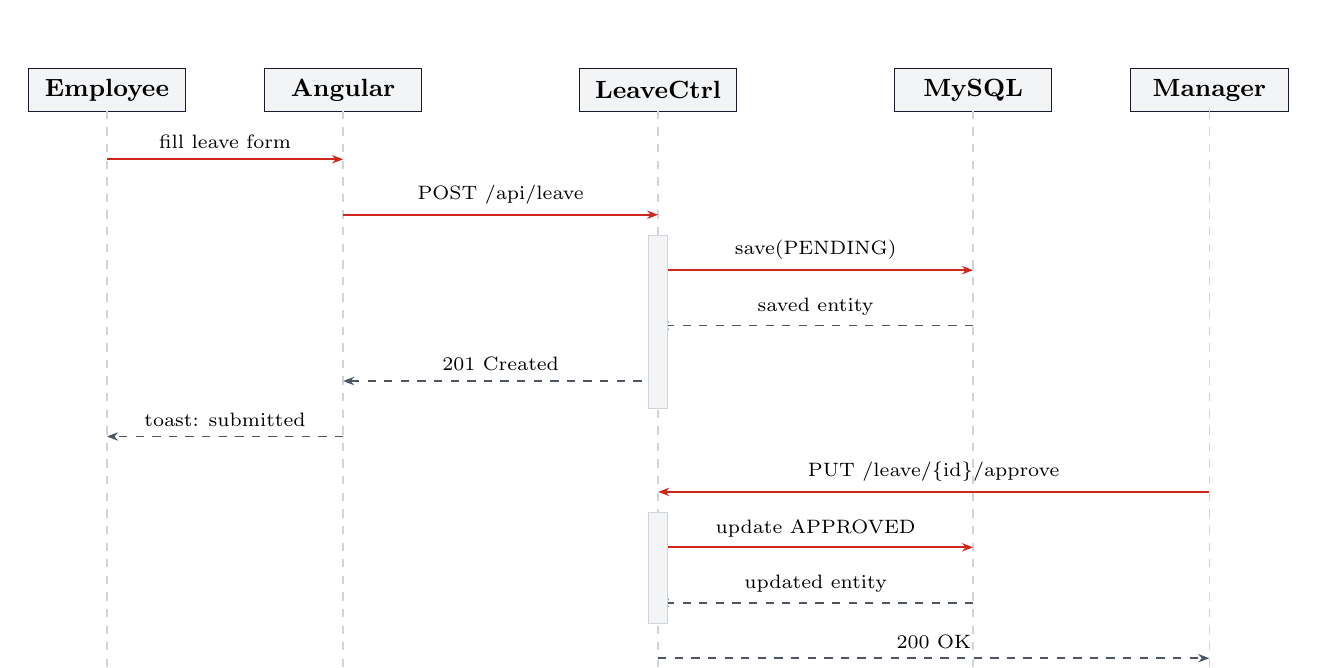
\begin{tikzpicture}[xscale=1.0, yscale=0.88]
  \node[seqobj] (emp) at (0.0,8) {Employee};
  \node[seqobj] (fe)  at (3.0,8) {Angular};
  \node[seqobj] (be)  at (7.0,8) {LeaveCtrl};
  \node[seqobj] (db)  at (11.0,8){MySQL};
  \node[seqobj] (mgr) at (14.0,8){Manager};

  \foreach \x in {0,3,7,11,14}
    \draw[draw=adpborder,dashed,line width=0.5pt] (\x,7.7) -- (\x,-0.5);

  \draw[seqmsg] (0,7.0)  -- (3,7.0)
    node[midway,above,font=\scriptsize]{fill leave form};
  \draw[seqmsg] (3,6.2)  -- (7,6.2)
    node[midway,above,font=\scriptsize]{POST /api/leave};
  \draw[seqmsg] (7,5.4)  -- (11,5.4)
    node[midway,above,font=\scriptsize]{save(PENDING)};
  \draw[seqret] (11,4.6) -- (7,4.6)
    node[midway,above,font=\scriptsize]{saved entity};
  \draw[seqret] (7,3.8)  -- (3,3.8)
    node[midway,above,font=\scriptsize]{201 Created};
  \draw[seqret] (3,3.0)  -- (0,3.0)
    node[midway,above,font=\scriptsize]{toast: submitted};

  \draw[seqmsg] (14,2.2) -- (7,2.2)
    node[midway,above,font=\scriptsize]{PUT /leave/\{id\}/approve};
  \draw[seqmsg] (7,1.4)  -- (11,1.4)
    node[midway,above,font=\scriptsize]{update APPROVED};
  \draw[seqret] (11,0.6) -- (7,0.6)
    node[midway,above,font=\scriptsize]{updated entity};
  \draw[seqret] (7,-0.2) -- (14,-0.2)
    node[midway,above,font=\scriptsize]{200 OK};

  \fill[adplightgray,draw=adpborder,line width=0.5pt]
    (6.88,5.9) rectangle (7.12,3.4);
  \fill[adplightgray,draw=adpborder,line width=0.5pt]
    (6.88,1.9) rectangle (7.12,0.3);
\end{tikzpicture}
\caption{Sequence Diagram, Leave Request Submission and Approval}
\label{fig:seq_leave}
\end{figure}

\subsection{AI Report Generation Sequence}

\begin{figure}[H]
\centering
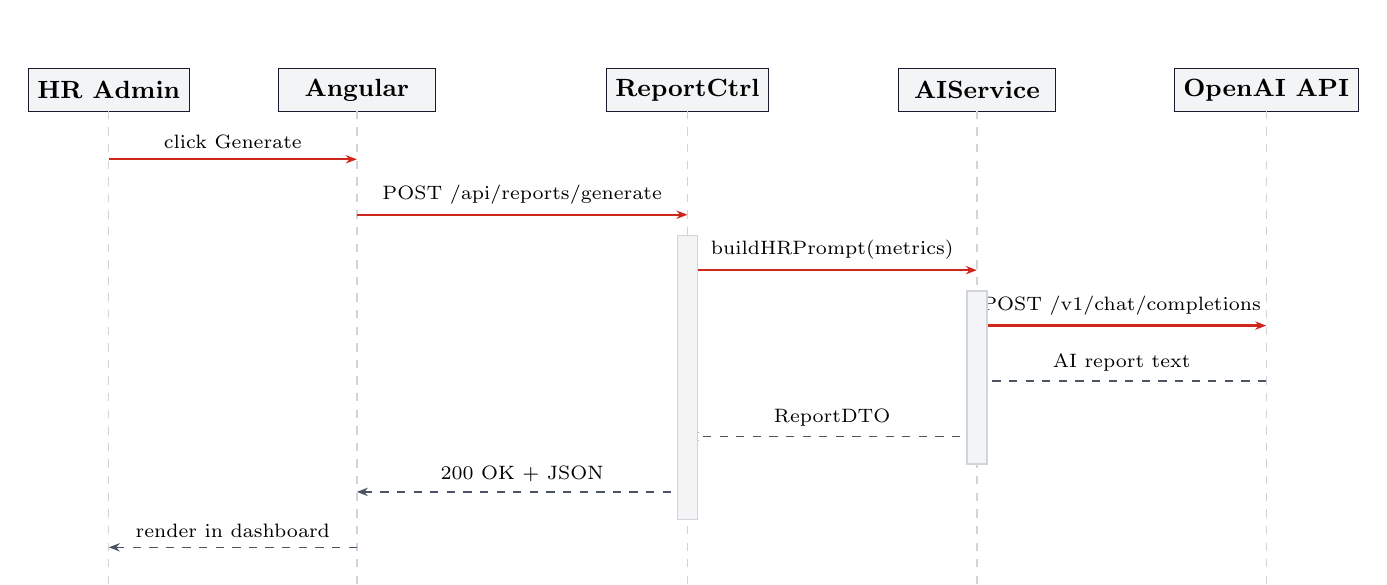
\begin{tikzpicture}[xscale=1.05, yscale=0.88]
  \node[seqobj] (admin) at (0.0,7) {HR Admin};
  \node[seqobj] (fe)    at (3.0,7) {Angular};
  \node[seqobj] (be)    at (7.0,7) {ReportCtrl};
  \node[seqobj] (svc)   at (10.5,7){AIService};
  \node[seqobj] (oai)   at (14.0,7){OpenAI API};

  \foreach \x in {0,3,7,10.5,14}
    \draw[draw=adpborder,dashed,line width=0.5pt] (\x,6.7) -- (\x,-0.3);

  \draw[seqmsg] (0,6.0)    -- (3,6.0)
    node[midway,above,font=\scriptsize]{click Generate};
  \draw[seqmsg] (3,5.2)    -- (7,5.2)
    node[midway,above,font=\scriptsize]{POST /api/reports/generate};
  \draw[seqmsg] (7,4.4)    -- (10.5,4.4)
    node[midway,above,font=\scriptsize]{buildHRPrompt(metrics)};
  \draw[seqmsg] (10.5,3.6) -- (14,3.6)
    node[midway,above,font=\scriptsize]{POST /v1/chat/completions};
  \draw[seqret] (14,2.8)   -- (10.5,2.8)
    node[midway,above,font=\scriptsize]{AI report text};
  \draw[seqret] (10.5,2.0) -- (7,2.0)
    node[midway,above,font=\scriptsize]{ReportDTO};
  \draw[seqret] (7,1.2)    -- (3,1.2)
    node[midway,above,font=\scriptsize]{200 OK + JSON};
  \draw[seqret] (3,0.4)    -- (0,0.4)
    node[midway,above,font=\scriptsize]{render in dashboard};

  \fill[adplightgray,draw=adpborder,line width=0.5pt]
    (6.88,4.9) rectangle (7.12,0.8);
  \fill[adplightgray,draw=adpborder,line width=0.5pt]
    (10.38,4.1) rectangle (10.62,1.6);
\end{tikzpicture}
\caption{Sequence Diagram, AI-Powered HR Report Generation}
\label{fig:seq_ai}
\end{figure}

\section{Database Schema}

\subsection{Entity-Relationship Diagram}

\begin{figure}[H]
\centering
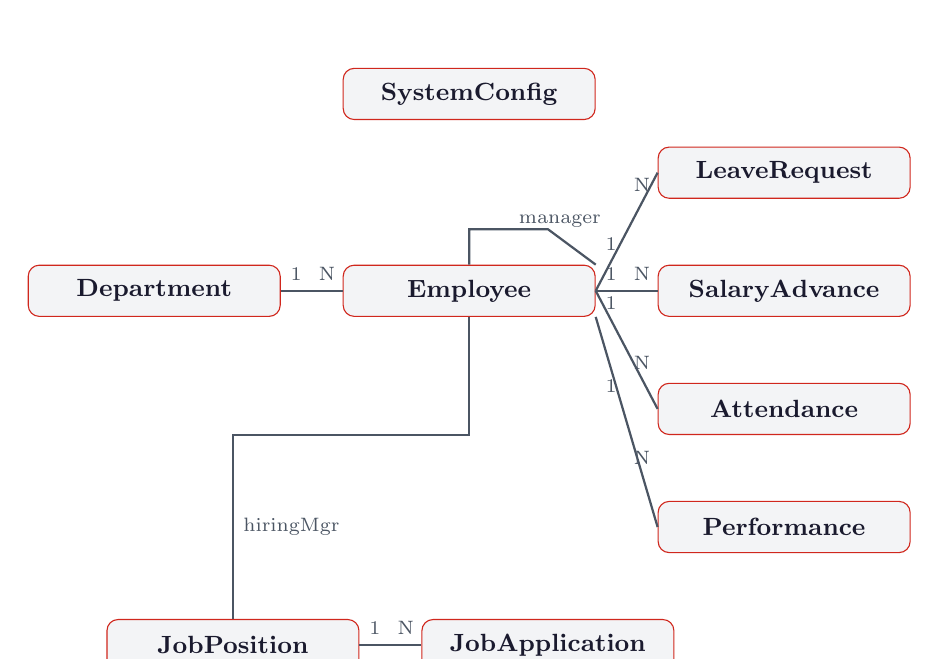
\begin{tikzpicture}[
  ent/.style={draw=adpred, fill=adplightgray, rounded corners=4pt,
              minimum width=3.2cm, minimum height=0.65cm,
              align=center, font=\small\bfseries\color{adpdark}},
  rel/.style={draw=adpgray, line width=0.8pt},
  card/.style={font=\scriptsize\color{adpgray}}
]
  \node[ent] (emp)    at (4.5,7.0) {Employee};
  \node[ent] (dept)   at (0.5,7.0) {Department};
  \node[ent] (leave)  at (8.5,8.5) {LeaveRequest};
  \node[ent] (adv)    at (8.5,7.0) {SalaryAdvance};
  \node[ent] (att)    at (8.5,5.5) {Attendance};
  \node[ent] (perf)   at (8.5,4.0) {Performance};
  \node[ent] (job)    at (1.5,2.5) {JobPosition};
  \node[ent] (app)    at (5.5,2.5) {JobApplication};
  \node[ent] (cfg)    at (4.5,9.5) {SystemConfig};

  \draw[rel] (emp.west)      -- (dept.east)
    node[near start,above,card]{N} node[near end,above,card]{1};
  \draw[rel] (emp.east)      -- (leave.west)
    node[near start,above,card]{1} node[near end,above,card]{N};
  \draw[rel] (emp.east)      -- (adv.west)
    node[near start,above,card]{1} node[near end,above,card]{N};
  \draw[rel] (emp.east)      -- (att.west)
    node[near start,above,card]{1} node[near end,above,card]{N};
  \draw[rel] (emp.south east) -- (perf.west)
    node[near start,below,card]{1} node[near end,above,card]{N};
  \draw[rel] (emp.south)    -- ++(0,-1.5) -| (job.north)
    node[near end,right,card]{hiringMgr};
  \draw[rel] (job.east)      -- (app.west)
    node[near start,above,card]{1} node[near end,above,card]{N};
  \draw[rel] (emp.north) -- ++(0,0.45) -| ++(1.0,0) -- (emp.north east)
    node[near start,above,card]{manager};

\end{tikzpicture}
\caption{Entity-Relationship Diagram, Nexus HCM}
\label{fig:erd}
\end{figure}

\subsection{Main Tables Description}

\begin{table}[H]
\centering
\caption{Main Database Tables}
\label{tab:db_tables}
\begin{tabular}{|C{3.6cm}|L{9.6cm}|}
\hline
\rowcolor{adplightgray}
\textbf{Table} & \textbf{Key Columns} \\
\hline
\textbf{employees} &
  id, first\_name, last\_name, email, password, role, status,
  department\_id (FK), manager\_id (self-FK) \\
\hline
\textbf{departments} &
  id, name, created\_at \\
\hline
\textbf{leave\_requests} &
  id, employee\_id (FK), type, start\_date, end\_date, reason,
  status, reviewed\_by (FK), notes \\
\hline
\textbf{salary\_advances} &
  id, employee\_id (FK), amount, reason, status,
  reviewed\_by (FK), notes, request\_date \\
\hline
\textbf{attendance} &
  id, employee\_id (FK), date, check\_in, check\_out \\
\hline
\textbf{performance\_evaluations} &
  id, employee\_id (FK), period, score, notes, evaluated\_by (FK) \\
\hline
\textbf{job\_positions} &
  id, title, description, requirements, department, location,
  job\_type, status, salary\_min, salary\_max, closing\_date,
  hiring\_manager\_id (FK) \\
\hline
\textbf{job\_applications} &
  id, position\_id (FK), applicant\_name, applicant\_email, phone,
  cover\_letter, cv\_file\_name, cv\_data, status, applied\_date \\
\hline
\textbf{system\_configs} &
  id, config\_key, config\_value, category \\
\hline
\end{tabular}
\end{table}

\section{Deployment Architecture}

\begin{figure}[H]
\centering
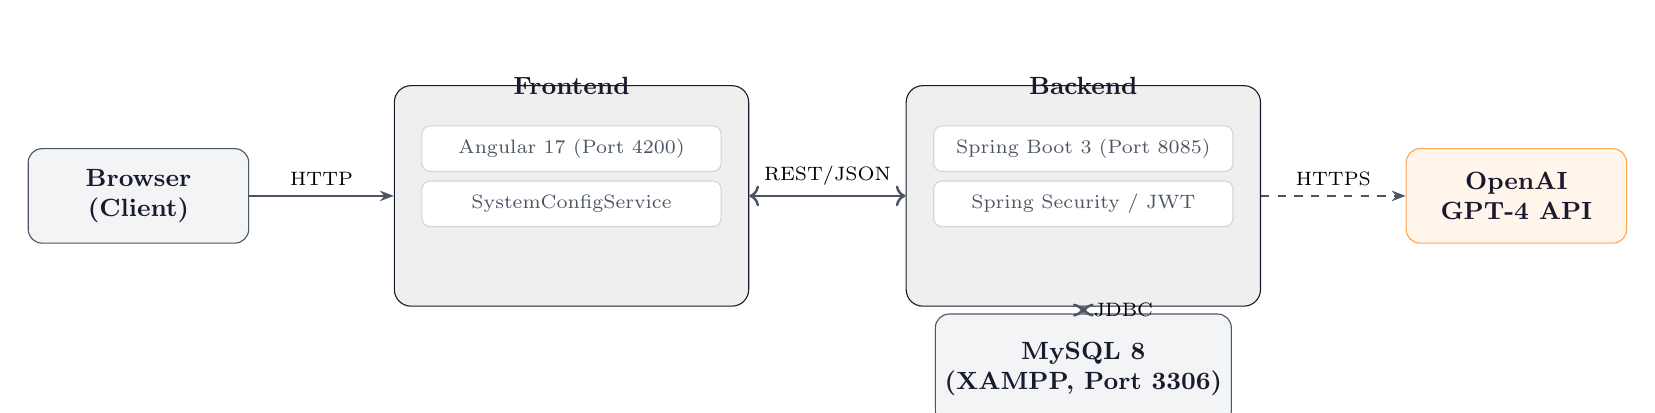
\begin{tikzpicture}[
  server/.style={draw=adpdark, fill=adpdark!7, rounded corners=6pt,
                 minimum width=4.5cm, minimum height=2.8cm,
                 align=center},
  comp/.style={draw=adpborder, fill=white, rounded corners=3pt,
               minimum width=3.8cm, minimum height=0.58cm,
               align=center, font=\scriptsize\color{adpgray}},
  conn/.style={draw=adpgray,line width=0.9pt,-{Stealth[length=5pt]}}
]
  \node[draw=adpgray,fill=adplightgray,rounded corners=5pt,
        minimum width=2.8cm, minimum height=1.2cm, align=center,
        font=\small\bfseries\color{adpdark}]
    (browser) at (-5.5,2.5) {Browser\\(Client)};

  \node[server] (fe) at (0,2.5) {};
  \node[font=\small\bfseries\color{adpdark}] at (0,3.9) {Frontend};
  \node[comp] at (0,3.1) {Angular 17 (Port 4200)};
  \node[comp] at (0,2.4) {SystemConfigService};

  \node[server] (be) at (6.5,2.5) {};
  \node[font=\small\bfseries\color{adpdark}] at (6.5,3.9) {Backend};
  \node[comp] at (6.5,3.1) {Spring Boot 3 (Port 8085)};
  \node[comp] at (6.5,2.4) {Spring Security / JWT};

  \node[draw=adpgray,fill=adplightgray,rounded corners=5pt,
        minimum width=3.4cm, minimum height=1.4cm, align=center,
        font=\small\bfseries\color{adpdark}]
    (db) at (6.5,0.3) {MySQL 8\\(XAMPP, Port 3306)};

  \node[draw=orange!70,fill=orange!8,rounded corners=5pt,
        minimum width=2.8cm, minimum height=1.2cm, align=center,
        font=\small\bfseries\color{adpdark}]
    (oai) at (12,2.5) {OpenAI\\GPT-4 API};

  \draw[conn] (browser.east) -- (fe.west)
    node[midway,above,font=\scriptsize]{HTTP};
  \draw[conn,<->] (fe.east) -- (be.west)
    node[midway,above,font=\scriptsize]{REST/JSON};
  \draw[conn,<->] (be.south) -- (db.north)
    node[midway,right,font=\scriptsize]{JDBC};
  \draw[conn,dashed] (be.east) -- (oai.west)
    node[midway,above,font=\scriptsize]{HTTPS};

\end{tikzpicture}
\caption{Nexus HCM, Deployment Architecture}
\label{fig:deployment}
\end{figure}

\section{Conclusion}

This chapter established the complete technical foundation of Nexus HCM. The three-tier
architecture ensures a clean separation of concerns between presentation, business logic,
and data. The UML class diagram formalizes all nine domain entities and their associations.
The sequence diagrams trace the critical flows (authentication, leave approval, AI report
generation), and the deployment diagram illustrates the runtime topology including the
external OpenAI API integration.

\newpage

%%=======================================================================
%% CHAPTER 4
%%=======================================================================
\chapter{Implementation}

\section{Introduction}

This chapter presents the practical implementation of Nexus HCM across four development
sprints. Each sprint section includes a backlog table, a description of the key technical
realizations, state machine or flow diagrams, and screenshot placeholders for the
delivered interfaces.

\section{Development Environment}

\begin{table}[H]
\centering
\caption{Development Environment}
\label{tab:dev_env}
\begin{tabular}{|C{3.5cm}|C{3.0cm}|L{6.5cm}|}
\hline
\rowcolor{adplightgray}
\textbf{Tool} & \textbf{Version} & \textbf{Purpose} \\
\hline
IntelliJ IDEA      & 2024.x    & Java / Spring Boot development \\
\hline
Visual Studio Code & 1.90+     & Angular / TypeScript development \\
\hline
XAMPP              & 8.2       & Local MySQL database server \\
\hline
Node.js            & 20 LTS    & Angular CLI and npm packages \\
\hline
Java JDK           & 21        & Spring Boot runtime \\
\hline
Git / GitHub       & 2.44      & Version control and collaboration \\
\hline
Postman            & 11.x      & REST API testing \\
\hline
\end{tabular}
\end{table}

\section{Sprint 1, Authentication and Employee Management}

\subsection{Sprint 1 Backlog}

\begin{table}[H]
\centering
\caption{Sprint 1 Backlog}
\label{tab:s1_backlog}
\begin{tabular}{|C{1.2cm}|L{7cm}|C{2cm}|C{2.5cm}|}
\hline
\rowcolor{adplightgray}
\textbf{ID} & \textbf{User Story} & \textbf{Priority} & \textbf{Status} \\
\hline
US-01 & As a user, I want to log in and be redirected to my role dashboard & High & \cmark Done \\
\hline
US-02 & As an HR Admin, I want to create employee accounts with activation email & High & \cmark Done \\
\hline
US-03 & As an HR Admin, I want to manage departments & Medium & \cmark Done \\
\hline
US-04 & As a new employee, I want to activate my account via email link & High & \cmark Done \\
\hline
US-05 & As an HR Admin, I want a dashboard with workforce KPIs & Medium & \cmark Done \\
\hline
\end{tabular}
\end{table}

\subsection{JWT Authentication}

The authentication flow relies on stateless JWT tokens. The backend validates credentials
using BCrypt password comparison, generates a signed JWT containing the user email and
role, and returns it to the client. The Angular frontend stores the token in
\texttt{localStorage} and attaches it to every subsequent request via an HTTP interceptor.
Route guards read the stored role to control access to protected routes.

\subsection{HR Admin Dashboard Overview}

The HR Admin dashboard is organized into five tabs and displays four real-time KPI cards
on the overview tab, summarizing the most critical workforce indicators.

\begin{table}[H]
\centering
\caption{HR Admin Dashboard, KPI Cards}
\label{tab:kpi_cards}
\begin{tabular}{|C{4cm}|L{9cm}|}
\hline
\rowcolor{adplightgray}
\textbf{KPI Card} & \textbf{Data Displayed} \\
\hline
Total Employees       & Count of all active employees \\
\hline
Pending Leave Requests & Requests awaiting HR or manager review \\
\hline
Present Today         & Employees who clocked in today \\
\hline
Pending Advances      & Salary advance requests awaiting approval \\
\hline
\end{tabular}
\end{table}

\begin{figure}[H]
\centering
\fbox{\parbox{0.88\textwidth}{\centering\vspace{2.8cm}
\textit{[Screenshot: HR Admin Dashboard, Overview Tab]}
\vspace{2.8cm}}}
\caption{HR Admin Dashboard, Overview Tab}
\label{fig:hr_dashboard}
\end{figure}

\begin{figure}[H]
\centering
\fbox{\parbox{0.88\textwidth}{\centering\vspace{2.8cm}
\textit{[Screenshot: Employee Management Interface]}
\vspace{2.8cm}}}
\caption{Employee Management Interface}
\label{fig:employees}
\end{figure}

\section{Sprint 2, HR Operations}

\subsection{Sprint 2 Backlog}

\begin{table}[H]
\centering
\caption{Sprint 2 Backlog}
\label{tab:s2_backlog}
\begin{tabular}{|C{1.2cm}|L{7cm}|C{2cm}|C{2.5cm}|}
\hline
\rowcolor{adplightgray}
\textbf{ID} & \textbf{User Story} & \textbf{Priority} & \textbf{Status} \\
\hline
US-06 & As an HR Admin, I want a collapsible org chart & High & \cmark Done \\
\hline
US-07 & As an employee, I want to submit leave requests & High & \cmark Done \\
\hline
US-08 & As a manager, I want to approve or reject leave requests & High & \cmark Done \\
\hline
US-09 & As an employee, I want to clock in and clock out & Medium & \cmark Done \\
\hline
US-10 & As an employee, I want to submit a salary advance request & Medium & \cmark Done \\
\hline
US-11 & As an HR Admin, I want to conduct performance evaluations & Medium & \cmark Done \\
\hline
\end{tabular}
\end{table}

\subsection{Organizational Chart Algorithm}

The org chart builds a flat display array from the hierarchical employee list using a
recursive \texttt{flatten()} traversal. Each node stores its depth level, ancestor
connector state (used to draw the vertical continuation lines), collapse state, and
direct report count. Toggling a node updates a \texttt{Set<number>} of collapsed IDs
and triggers a full tree rebuild, skipping children of collapsed nodes.

\begin{figure}[H]
\centering
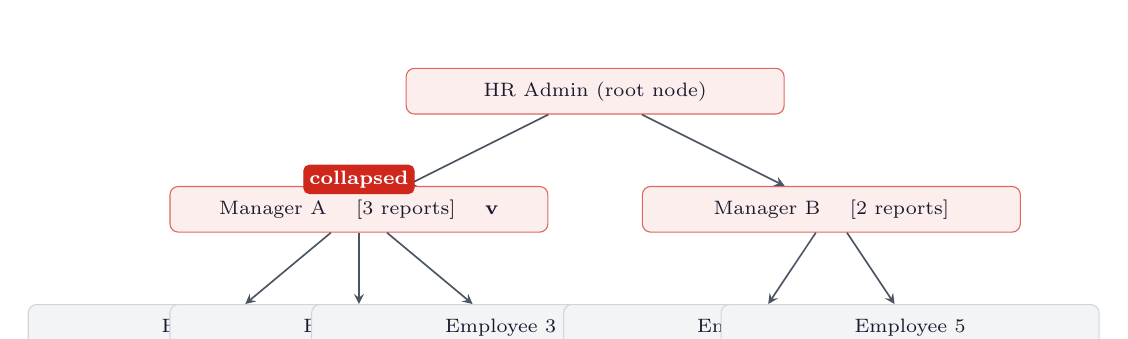
\begin{tikzpicture}[
  nd/.style={draw=adpborder, fill=adplightgray, rounded corners=3pt,
             minimum width=4.8cm, minimum height=0.58cm,
             align=center, font=\scriptsize\color{adpdark}},
  mgr/.style={draw=adpred!70, fill=adpred!8, rounded corners=3pt,
              minimum width=4.8cm, minimum height=0.58cm,
              align=center, font=\scriptsize\color{adpdark}},
  arr/.style={draw=adpgray, line width=0.6pt, -stealth}
]
  \node[mgr] (root) at (5,6.0) {HR Admin (root node)};
  \node[mgr] (m1)   at (2,4.5) {Manager A \quad [3 reports] \quad \textbf{v}};
  \node[mgr] (m2)   at (8,4.5) {Manager B \quad [2 reports]};
  \node[nd]  (e1)   at (0.2,3.0) {Employee 1};
  \node[nd]  (e2)   at (2.0,3.0) {Employee 2};
  \node[nd]  (e3)   at (3.8,3.0) {Employee 3};
  \node[nd]  (e4)   at (7.0,3.0) {Employee 4};
  \node[nd]  (e5)   at (9.0,3.0) {Employee 5};

  \draw[arr] (root) -- (m1);
  \draw[arr] (root) -- (m2);
  \draw[arr] (m1)   -- (e1);
  \draw[arr] (m1)   -- (e2);
  \draw[arr] (m1)   -- (e3);
  \draw[arr] (m2)   -- (e4);
  \draw[arr] (m2)   -- (e5);

  \node[draw=adpred,fill=adpred,text=white,rounded corners=2pt,
        font=\scriptsize\bfseries,inner sep=2pt]
    at (2.0,4.88) {collapsed};

\end{tikzpicture}
\caption{Organizational Chart, Collapsible Tree Visualization}
\label{fig:orgchart_diagram}
\end{figure}

\begin{figure}[H]
\centering
\fbox{\parbox{0.88\textwidth}{\centering\vspace{2.8cm}
\textit{[Screenshot: Organizational Chart, Expanded View]}
\vspace{2.8cm}}}
\caption{Organizational Chart Interface}
\label{fig:orgchart}
\end{figure}

\subsection{Leave Request Workflow}

\begin{figure}[H]
\centering
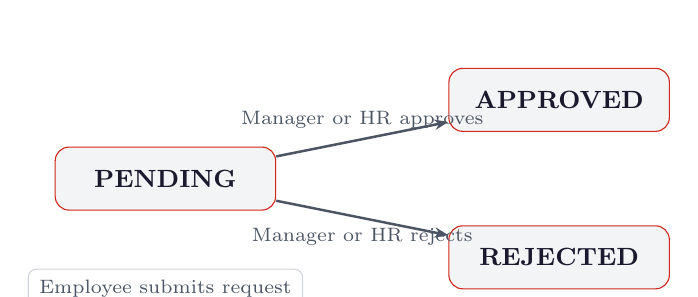
\begin{tikzpicture}[
  st/.style={draw=adpred, fill=adplightgray, rounded corners=5pt,
             minimum width=2.8cm, minimum height=0.8cm,
             align=center, font=\small\bfseries\color{adpdark}},
  arr/.style={-{Stealth[length=5pt]},draw=adpgray,line width=0.9pt}
]
  \node[st] (p) at (0,0)    {PENDING};
  \node[st] (a) at (5.0,1.0){APPROVED};
  \node[st] (r) at (5.0,-1.0){REJECTED};

  \draw[arr] (p) -- node[above,font=\scriptsize\color{adpgray}]
    {Manager or HR approves} (a);
  \draw[arr] (p) -- node[below,font=\scriptsize\color{adpgray}]
    {Manager or HR rejects} (r);

  \node[draw=adpborder,fill=white,rounded corners=3pt,
        font=\scriptsize\color{adpgray},inner sep=4pt]
    at (0,-1.4) {Employee submits request};
\end{tikzpicture}
\caption{Leave Request State Machine}
\label{fig:leave_state}
\end{figure}

\begin{figure}[H]
\centering
\fbox{\parbox{0.88\textwidth}{\centering\vspace{2.8cm}
\textit{[Screenshot: Leave Request Management Tab]}
\vspace{2.8cm}}}
\caption{Leave Request Management Interface}
\label{fig:leave_ui}
\end{figure}

\section{Sprint 3, Recruitment and AI Integration}

\subsection{Sprint 3 Backlog}

\begin{table}[H]
\centering
\caption{Sprint 3 Backlog}
\label{tab:s3_backlog}
\begin{tabular}{|C{1.2cm}|L{7cm}|C{2cm}|C{2.5cm}|}
\hline
\rowcolor{adplightgray}
\textbf{ID} & \textbf{User Story} & \textbf{Priority} & \textbf{Status} \\
\hline
US-12 & As an HR Admin, I want to create and publish job positions & High & \cmark Done \\
\hline
US-13 & As a candidate, I want to browse open positions and apply & High & \cmark Done \\
\hline
US-14 & As a candidate, I want to attach my CV to my application & Medium & \cmark Done \\
\hline
US-15 & As an HR Admin, I want AI to score each application & High & \cmark Done \\
\hline
US-16 & As an HR Admin, I want to generate an AI HR report & High & \cmark Done \\
\hline
US-17 & As an HR Admin, I want to configure platform branding live & Medium & \cmark Done \\
\hline
\end{tabular}
\end{table}

\subsection{Job Position and Application Pipelines}

\begin{figure}[H]
\centering
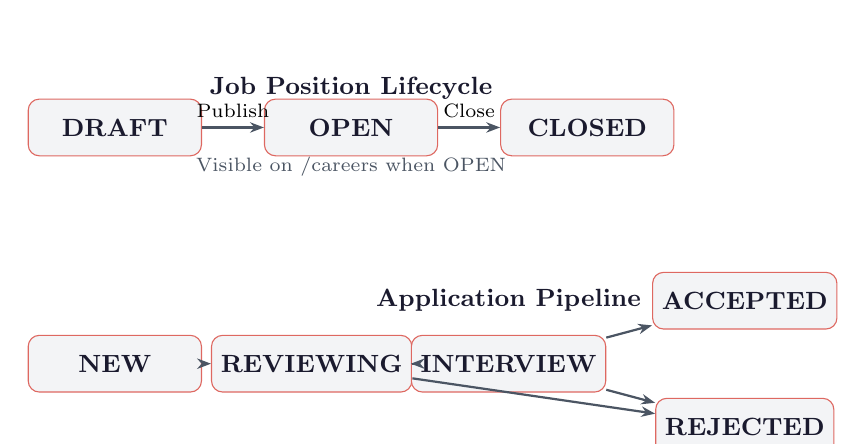
\begin{tikzpicture}[
  st/.style={draw=adpred!70, fill=adplightgray, rounded corners=4pt,
             minimum width=2.2cm, minimum height=0.72cm,
             align=center, font=\small\bfseries\color{adpdark}},
  arr/.style={-{Stealth[length=5pt]},draw=adpgray,line width=0.8pt}
]
  %% Position lifecycle
  \node[font=\small\bfseries\color{adpdark}] at (3,2.5) {Job Position Lifecycle};
  \node[st] (d) at (0,2.0)  {DRAFT};
  \node[st] (o) at (3,2.0)  {OPEN};
  \node[st] (c) at (6,2.0)  {CLOSED};
  \draw[arr] (d) -- node[above,font=\scriptsize]{Publish} (o);
  \draw[arr] (o) -- node[above,font=\scriptsize]{Close}   (c);
  \node[font=\scriptsize\color{adpgray}] at (3,1.5)
    {Visible on /careers when OPEN};

  %% Application pipeline
  \node[font=\small\bfseries\color{adpdark}] at (5,-0.2) {Application Pipeline};
  \node[st] (n)  at (0,-1.0) {NEW};
  \node[st] (rv) at (2.5,-1.0){REVIEWING};
  \node[st] (iv) at (5,-1.0) {INTERVIEW};
  \node[st] (ac) at (8.0,-0.2){ACCEPTED};
  \node[st] (rj) at (8.0,-1.8){REJECTED};
  \draw[arr] (n)  -- (rv);
  \draw[arr] (rv) -- (iv);
  \draw[arr] (iv) -- (ac);
  \draw[arr] (iv) -- (rj);
  \draw[arr] (rv) -- (rj);
\end{tikzpicture}
\caption{Job Position Lifecycle and Application Pipeline}
\label{fig:pipelines}
\end{figure}

\subsection{AI Integration}

\subsubsection{AI-Powered HR Report Generation}

When the HR Admin triggers report generation, the backend aggregates current workforce
metrics and constructs a structured prompt containing employee counts by department, leave
approval rates, attendance statistics, and open positions. This prompt is sent to the
OpenAI GPT-4 Chat Completions API via HTTPS. The returned natural-language text is
rendered directly in the dashboard as an executive HR summary.

\subsubsection{Intelligent CV Screening}

When a new application arrives, the backend pairs the applicant's cover letter text with
the job requirements in a scoring prompt and submits it to the AI API. The response
contains a match score from 0 to 100 and highlights matching skills and identified gaps.
This score appears as a badge next to each application row in the HR panel, enabling
rapid shortlisting without manual reading of every cover letter.

\begin{figure}[H]
\centering
\fbox{\parbox{0.88\textwidth}{\centering\vspace{2.8cm}
\textit{[Screenshot: Job Board, Applications with AI Screening Scores]}
\vspace{2.8cm}}}
\caption{Job Board, Application List with AI Screening Score Badges}
\label{fig:job_board}
\end{figure}

\begin{figure}[H]
\centering
\fbox{\parbox{0.88\textwidth}{\centering\vspace{2.8cm}
\textit{[Screenshot: Public Careers Page]}
\vspace{2.8cm}}}
\caption{Public Careers Page with Position Listings}
\label{fig:careers}
\end{figure}

\section{Sprint 4, Polish and Deployment}

\subsection{Sprint 4 Backlog}

\begin{table}[H]
\centering
\caption{Sprint 4 Backlog}
\label{tab:s4_backlog}
\begin{tabular}{|C{1.2cm}|L{7cm}|C{2cm}|C{2.5cm}|}
\hline
\rowcolor{adplightgray}
\textbf{ID} & \textbf{User Story} & \textbf{Priority} & \textbf{Status} \\
\hline
US-18 & As an HR Admin, I want a full audit trail of platform actions & High & \cmark Done \\
\hline
US-19 & As a manager, I want a dedicated team supervision dashboard & High & \cmark Done \\
\hline
US-20 & As an employee, I want a personal self-service portal & Medium & \cmark Done \\
\hline
US-21 & TypeScript compilation returns 0 errors across the codebase & High & \cmark Done \\
\hline
US-22 & All source code deployed to GitHub with descriptive commits & Medium & \cmark Done \\
\hline
\end{tabular}
\end{table}

\subsection{Dynamic System Configuration}

The \texttt{SystemConfigService} loads platform branding from \texttt{/api/config/public}
at application startup via Angular's \texttt{APP\_INITIALIZER}. It caches the values and
writes them as CSS custom properties on the document root element. This means that when
an HR Admin updates the company name, logo URL, or primary color, the change propagates
in real time to every page, including the public login and Careers pages, without any
server restart.

\begin{figure}[H]
\centering
\fbox{\parbox{0.88\textwidth}{\centering\vspace{2.8cm}
\textit{[Screenshot: System Configuration Panel]}
\vspace{2.8cm}}}
\caption{System Configuration, Live Branding Management}
\label{fig:sysconfig}
\end{figure}

\section{Feature Access Matrix}

\begin{table}[H]
\centering
\caption{Feature Access Matrix by Role}
\label{tab:feature_matrix}
\begin{tabular}{|L{4.5cm}|C{2.2cm}|C{2.2cm}|C{2.2cm}|C{1.5cm}|}
\hline
\rowcolor{adplightgray}
\textbf{Feature} & \textbf{HR Admin} & \textbf{Manager} & \textbf{Employee} & \textbf{Public} \\
\hline
Authentication            & \cmark & \cmark & \cmark &,    \\
\hline
Employee Management       & \cmark &,    &,    &,    \\
\hline
Department Management     & \cmark &,    &,    &,    \\
\hline
Org Chart                 & \cmark & \cmark &,    &,    \\
\hline
Leave Management          & \cmark & \cmark & \cmark &,    \\
\hline
Attendance Tracking       & \cmark & \cmark & \cmark &,    \\
\hline
Performance Evaluation    & \cmark & \cmark &,    &,    \\
\hline
Salary Advance Requests   & \cmark &,    & \cmark &,    \\
\hline
Job Board (Admin Panel)   & \cmark &,    &,    &,    \\
\hline
Careers Page              &,    &,    &,    & \cmark \\
\hline
AI Report Generation      & \cmark &,    &,    &,    \\
\hline
System Configuration      & \cmark &,    &,    &,    \\
\hline
\end{tabular}
\end{table}

\section{Conclusion}

This chapter described the implementation of Nexus HCM across four development sprints.
Each sprint was driven by a prioritized backlog and validated with the company supervisor
through sprint review meetings. The platform delivers all functional requirements identified
in Chapter 2 with a coherent, role-specific user experience and AI-powered capabilities
that elevate it beyond a conventional HR management system.

\newpage

%%=======================================================================
%% CHAPTER 5
%%=======================================================================
\chapter{Testing and Validation}

\section{Introduction}

This chapter presents the testing strategy and validation results for the Nexus HCM
platform. It covers the levels of testing performed, the tools used, and the outcomes
obtained, demonstrating that the delivered system meets the requirements specified
in Chapter 2.

\section{Testing Strategy}

The testing approach followed a multi-level strategy aligned with the sprint cadence.

\begin{figure}[H]
\centering
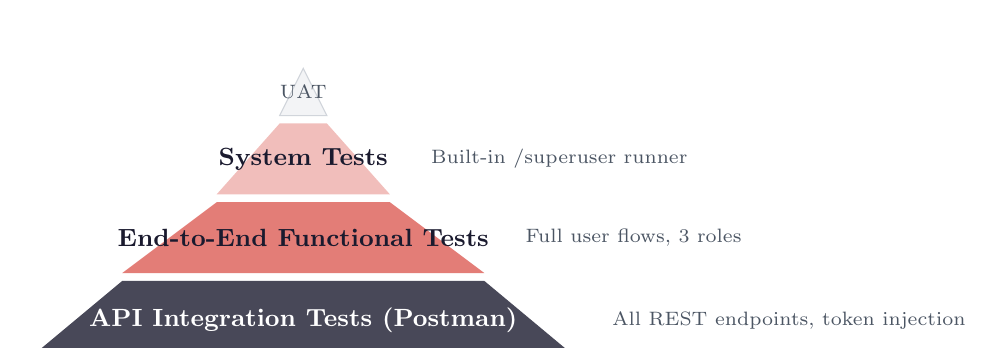
\begin{tikzpicture}
  %% Pyramid
  \fill[adpdark!80] (0,0)   -- (7,0)   -- (5.8,1.0) -- (1.2,1.0) -- cycle;
  \fill[adpred!60]  (1.2,1.1)-- (5.8,1.1)-- (4.6,2.0)-- (2.4,2.0)-- cycle;
  \fill[adpred!30]  (2.4,2.1)-- (4.6,2.1)-- (3.8,3.0)-- (3.2,3.0)-- cycle;
  \fill[adplightgray,draw=adpborder]
                    (3.2,3.1)-- (3.8,3.1)-- (3.5,3.7)-- cycle;

  \node[text=white,  font=\small\bfseries,align=center] at (3.5,0.5)
    {API Integration Tests (Postman)};
  \node[text=adpdark,font=\small\bfseries,align=center] at (3.5,1.55)
    {End-to-End Functional Tests};
  \node[text=adpdark,font=\small\bfseries,align=center] at (3.5,2.55)
    {System Tests};
  \node[font=\scriptsize\color{adpgray}] at (3.5,3.4) {UAT};

  \node[right=0.3cm,font=\scriptsize\color{adpgray}] at (7.0,0.5)
    {All REST endpoints, token injection};
  \node[right=0.3cm,font=\scriptsize\color{adpgray}] at (5.9,1.55)
    {Full user flows, 3 roles};
  \node[right=0.3cm,font=\scriptsize\color{adpgray}] at (4.7,2.55)
    {Built-in /superuser runner};
\end{tikzpicture}
\caption{Testing Pyramid, Nexus HCM}
\label{fig:test_pyramid}
\end{figure}

\section{API Integration Tests}

All REST endpoints were tested using \textbf{Postman}. A dedicated collection with
automated JWT injection was built for this purpose.

\begin{table}[H]
\centering
\caption{API Test Results}
\label{tab:api_tests}
\begin{tabular}{|L{5.2cm}|C{1.8cm}|C{2cm}|C{2cm}|C{1.4cm}|}
\hline
\rowcolor{adplightgray}
\textbf{Test Case} & \textbf{Method} & \textbf{Expected} & \textbf{Result} & \textbf{Status} \\
\hline
Login with valid credentials    & POST & 200 + JWT & 200 + JWT & \cmark \\
\hline
Login with wrong password       & POST & 401       & 401       & \cmark \\
\hline
Get employees without token     & GET  & 403       & 403       & \cmark \\
\hline
Create employee (HR Admin)      & POST & 200       & 200       & \cmark \\
\hline
Create employee (Manager role)  & POST & 403       & 403       & \cmark \\
\hline
Approve leave request           & PUT  & 200       & 200       & \cmark \\
\hline
Submit application (public)     & POST & 200       & 200       & \cmark \\
\hline
Get open positions (no token)   & GET  & 200       & 200       & \cmark \\
\hline
Publish job position            & PUT  & 200       & 200       & \cmark \\
\hline
Update application status       & PUT  & 200       & 200       & \cmark \\
\hline
\end{tabular}
\end{table}

\section{Functional Tests}

End-to-end functional tests were performed manually for each user role, verifying complete
interaction flows from login through feature execution.

\begin{table}[H]
\centering
\caption{Functional Test Results}
\label{tab:func_tests}
\begin{tabular}{|L{5.5cm}|C{2.4cm}|L{4.8cm}|}
\hline
\rowcolor{adplightgray}
\textbf{Test Scenario} & \textbf{Role} & \textbf{Result} \\
\hline
Login, role-based redirection          & All      & \cmark Correct dashboard \\
\hline
Create employee, activation email sent & HR Admin & \cmark Email triggered \\
\hline
Assign employee to department          & HR Admin & \cmark Reflected in table \\
\hline
Collapse/expand org chart node         & HR Admin & \cmark Subtree hidden/shown \\
\hline
Submit leave request                   & Employee & \cmark Status PENDING \\
\hline
Approve leave request                  & Manager  & \cmark Status APPROVED \\
\hline
Salary advance full cycle              & Emp/HR   & \cmark Request, review, decision \\
\hline
Publish job, visible on /careers       & HR Admin & \cmark Position appears publicly \\
\hline
Apply with CV on Careers page          & Public   & \cmark Application stored \\
\hline
AI CV screening score visible          & HR Admin & \cmark Score badge shown \\
\hline
Generate AI HR report                  & HR Admin & \cmark Report displayed \\
\hline
Change branding, propagates live       & HR Admin & \cmark All pages updated \\
\hline
\end{tabular}
\end{table}

\section{Built-in System Test Runner}

A dedicated \textbf{Superuser Dashboard} at \texttt{/superuser} was developed as an
internal regression test suite. It runs automated tests against the live backend,
each reporting PASS, WARN, or FAIL with detailed output.

\begin{table}[H]
\centering
\caption{Built-in Superuser Test Suite}
\label{tab:test_suite}
\begin{tabular}{|C{1.8cm}|L{5cm}|C{2.5cm}|C{3cm}|}
\hline
\rowcolor{adplightgray}
\textbf{Test ID} & \textbf{Description} & \textbf{Category} & \textbf{Pass Condition} \\
\hline
a1 & Login as HR Admin       & Authentication & role = HR\_ADMIN \\
\hline
a2 & Login as Manager        & Authentication & role = MANAGER \\
\hline
a3 & Login as Employee       & Authentication & role = EMPLOYEE \\
\hline
e1 & List all employees      & Employees      & HTTP 200, non-empty \\
\hline
e3 & Quick-create then delete & Employees     & Created, auto-cleaned \\
\hline
d1 & List departments        & Departments    & HTTP 200, non-empty \\
\hline
l1 & List leave requests     & Leave          & HTTP 200 \\
\hline
j1 & List open positions     & Job Board      & HTTP 200 \\
\hline
\end{tabular}
\end{table}

\section{TypeScript Validation}

After every development session, the Angular TypeScript compiler was run in no-emit mode
to detect type errors before any browser test:

\begin{lstlisting}[language=bash, caption={TypeScript Zero-Error Validation}]
npx tsc --noEmit --project tsconfig.app.json
# Result: 0 errors
\end{lstlisting}

\section{Conclusion}

The multi-level testing campaign confirmed that Nexus HCM satisfies all functional and
non-functional requirements. API endpoints respond correctly under valid and invalid
conditions, role-based access is consistently enforced end-to-end, and all user
workflows produce the expected outcomes across the four actor types. The built-in
superuser test runner provides ongoing regression coverage as the platform evolves.

\newpage

%%=======================================================================
%% GENERAL CONCLUSION
%%=======================================================================
\chapter*{General Conclusion and Perspectives}
\addcontentsline{toc}{chapter}{General Conclusion and Perspectives}

This end-of-studies internship at \textbf{ADP ES Tunisie} (April, September 2026)
resulted in the successful design, development, and validation of \textbf{Nexus HCM},
an Intelligent Human Capital Management System. The platform unifies and automates
the full HR lifecycle of an enterprise within a single, role-driven web application.

\textbf{Technical achievements} of this project include:

\begin{itemize}
  \item A complete \textbf{Spring Boot 3 / Java 21 REST API} with stateless JWT
    authentication, layered architecture, and Hibernate-managed MySQL persistence.
  \item A modern \textbf{Angular 17 standalone-component frontend} with three dedicated
    role dashboards, a public Careers page, and a real-time dynamic branding system.
  \item A full \textbf{recruitment module} covering job posting lifecycle management,
    a public candidate application flow with CV upload, and an HR application pipeline.
  \item An interactive \textbf{collapsible organizational chart} powered by a recursive
    tree-building algorithm with \texttt{FlatNode} structure.
  \item \textbf{AI integration via OpenAI GPT-4}: one-click executive HR report
    generation and intelligent CV screening with 0, 100 match scoring.
  \item A \textbf{built-in regression test suite} providing automated backend validation
    with granular PASS/WARN/FAIL reporting.
\end{itemize}

\textbf{Skills developed} during this internship include designing a full-stack
architecture from scratch, managing a six-month development project with Agile sprints,
communicating requirements with non-technical stakeholders, and maintaining consistent
code quality throughout a large, multi-module codebase.

\textbf{Future perspectives} for the Nexus HCM platform include:

\begin{itemize}
  \item \textbf{Payroll module:} automated payroll calculation based on attendance data,
    leave balances, and salary parameters.
  \item \textbf{Mobile application:} a React Native companion for employee self-service
    and clock-in/out on mobile devices.
  \item \textbf{Real-time analytics:} chart-based workforce dashboards using Chart.js
    or Apache ECharts.
  \item \textbf{Cloud deployment:} containerization with Docker and deployment on AWS
    or Azure for production readiness.
  \item \textbf{Advanced AI features:} employee churn prediction, skill gap analysis,
    and automated performance insights using historical HR data patterns.
  \item \textbf{Push notifications:} real-time in-app and email alerts for approvals,
    rejections, and HR broadcast messages.
\end{itemize}

\newpage

%%=======================================================================
%% REFERENCES
%%=======================================================================
\chapter*{References}
\addcontentsline{toc}{chapter}{References}

\begin{enumerate}[label={[\arabic*]}]
  \item Spring Framework Documentation.
    \textit{Spring Boot Reference Documentation 3.3}.
    \url{https://docs.spring.io/spring-boot/docs/3.3.x/reference/html/}.
    Accessed September 2026.

  \item Angular Team.
    \textit{Angular 17 Developer Guide, Standalone Components}.
    \url{https://angular.dev/guide/standalone-components}.
    Accessed September 2026.

  \item Oracle Corporation.
    \textit{Java SE 21 API Documentation}.
    \url{https://docs.oracle.com/en/java/javase/21/docs/api/}.
    Accessed April 2026.

  \item MySQL AB.
    \textit{MySQL 8.0 Reference Manual}.
    \url{https://dev.mysql.com/doc/refman/8.0/en/}.
    Accessed April 2026.

  \item Walls, C.
    \textit{Spring in Action, 6th Edition}.
    Manning Publications, 2022.

  \item OpenAI.
    \textit{Chat Completions API Reference}.
    \url{https://platform.openai.com/docs/api-reference/chat}.
    Accessed June 2026.

  \item ADP.
    \textit{About ADP, Company Overview}.
    \url{https://www.adp.com/about-adp.aspx}.
    Accessed March 2026.

  \item Auth0.
    \textit{JSON Web Token Introduction}.
    \url{https://jwt.io/introduction}.
    Accessed April 2026.

  \item Sommerville, I.
    \textit{Software Engineering, 10th Edition}.
    Pearson, 2015.

  \item Fowler, M.
    \textit{Patterns of Enterprise Application Architecture}.
    Addison-Wesley, 2002.
\end{enumerate}

\end{document}
